%*****************************************************************
%*************************** Section 4 ***************************
%********************* Antrieb des Fahrzeugs *********************
%*****************************************************************


\pagestyle{fancy}
\rhead{\thepage} \chead{} \lhead{\ref{Sec4}. \nameref{Sec4}}
\cfoot{}

\section{Antrieb des Fahrzeugs}\label{Sec4}

Wie in Kapitel \ref{Sec2Sub1} beschrieben, wird das Fahrzeug von zwei \acp{BLDCMot} angetrieben, die im Folgenden genauer erklärt werden. Zusätzlich dazu wird in diesem Kapitel auch näher auf die Montage der Antriebskomponenten, die Programmierung des Antriebsbausteins, die Konfiguration der Motorcontroller und die Drehzahlmessung eingegangen.

\subsection{BLDC-Antrieb und Motorcontroller}\label{Sec4Sub1}

\acp{BLDCMot} sind im Wesentlichen wie permanent erregte Synchronmaschinen aufgebaut. Sie besitzen Magnete im Rotor und Einzelzahnwicklungen im Stator. Da solche Motoren häufig im \ac{RC}-Bereich Einsatz finden, gibt es zu deren Ansteuerung bereits vorgefertigte Bausteine, sogenannte \ac{ESC}. Diese haben zwei Signalpins für ein \ac{PWM}-Signal und zwei Anschlüsse zur Spannungsversorgung des Motorcontrollers, aus welchen die drei Strangspannungen für die Phasen des Antriebs generiert werden. Aus diesen Strangspannungen kann im übrigen auch die Motordrehzahl ermittelt werden, was im Rahmen dieser Projektarbeit auch eines der Ziele darstellt. An den Signalpins wird ein \ac{PWM}-Signal mit einer Frequenz von 50Hz angelegt, dessen Pulsbreite zwischen 1ms und 2ms liegen darf. Daraus resultiert ein Tastgrad zwischen 5\% (Stillstand) und 10\% (maximal erreichbare Drehzahl). Die maximale Drehzahl des Antriebs hängt von der Spannung des Akkus ab. Je geringer diese Spannung ist, desto geringer ist die maximal erreichbare Drehzahl. Der Anschluss der Motoren erfolgt nach der in Abbildung \ref{fig:SkizzeAntrieb} gezeigten Weise.

\begin{figure}[H] %H für Positionierung hier
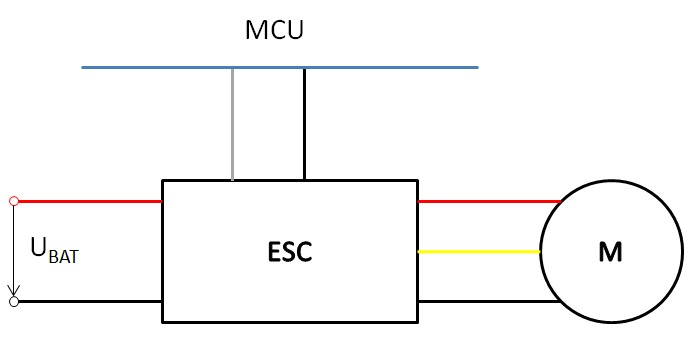
\includegraphics[width=.90\textwidth]{sec4/images/Skizze_BLDC_ESC} 
\centering
\captionsetup{width=.95\textwidth}
\caption[Skizze zur Beschaltung eines \ac{ESC}s und \ac{BLDCMot}s]{Skizze zur Beschaltung eines \ac{ESC}s und \ac{BLDCMot}s; Versorgungsspannung des \ac{ESC}s in rot und schwarz (Masse), \ac{PWM}-Signalleitungen in grau und schwarz (Masse) und Anschlussleitungen des \ac{BLDCMot}s in rot, gelb und schwarz}\centering
\label{fig:SkizzeAntrieb}
\end{figure}

\subsection{Montage der Antriebskomponenten}\label{Sec4Sub2}

Die Komponenten des Fahrzeugantriebs, welcher über zwei \acp{BLDCMot} realisiert ist, sind auf der unteren Fahrzeugebene montiert. Die Motoren selbst sind mit zwei Schrauben an der Karosserie befestigt. An der Welle der Motoren befindet sich je ein Zahnrad mit 13 Zähnen, welches ein weiteres Zahnrad mit 90 Zähnen antreibt, das an der Antriebswelle befestigt ist. Das heißt, dass sich die Reifen bei 6,923 Umdrehungen der Motorwelle genau einmal drehen.\vspace{11pt}

In Abbildung \ref{fig:MontageMotorUebersetzung} sind die montierten Komponenten des linken Antriebs abgebildet. Die Befestigungsschrauben der Motoren sind dabei in rot hervorgehoben, die Befestigungsschrauben des Zahnrads der Antriebswelle in blau und die Befestigung des Reifens in orange. Das Zahnrad der Motorwelle ist durch Erhitzen geweitet und auf die Welle aufgesetzt worden. Zur Sicherheit dient hier etwas Sekundenkleber dazu, dass sich das Zahnrad auf der Welle nicht durchdreht. Sekundenkleber ist hier völlig ausreichend, da aufgrund der Übersetzung nur 1/7 des auf die Reifen wirkenden Moments auf das Zahnrad der Motorwelle wirkt.

\begin{figure}[H] %H für Positionierung hier
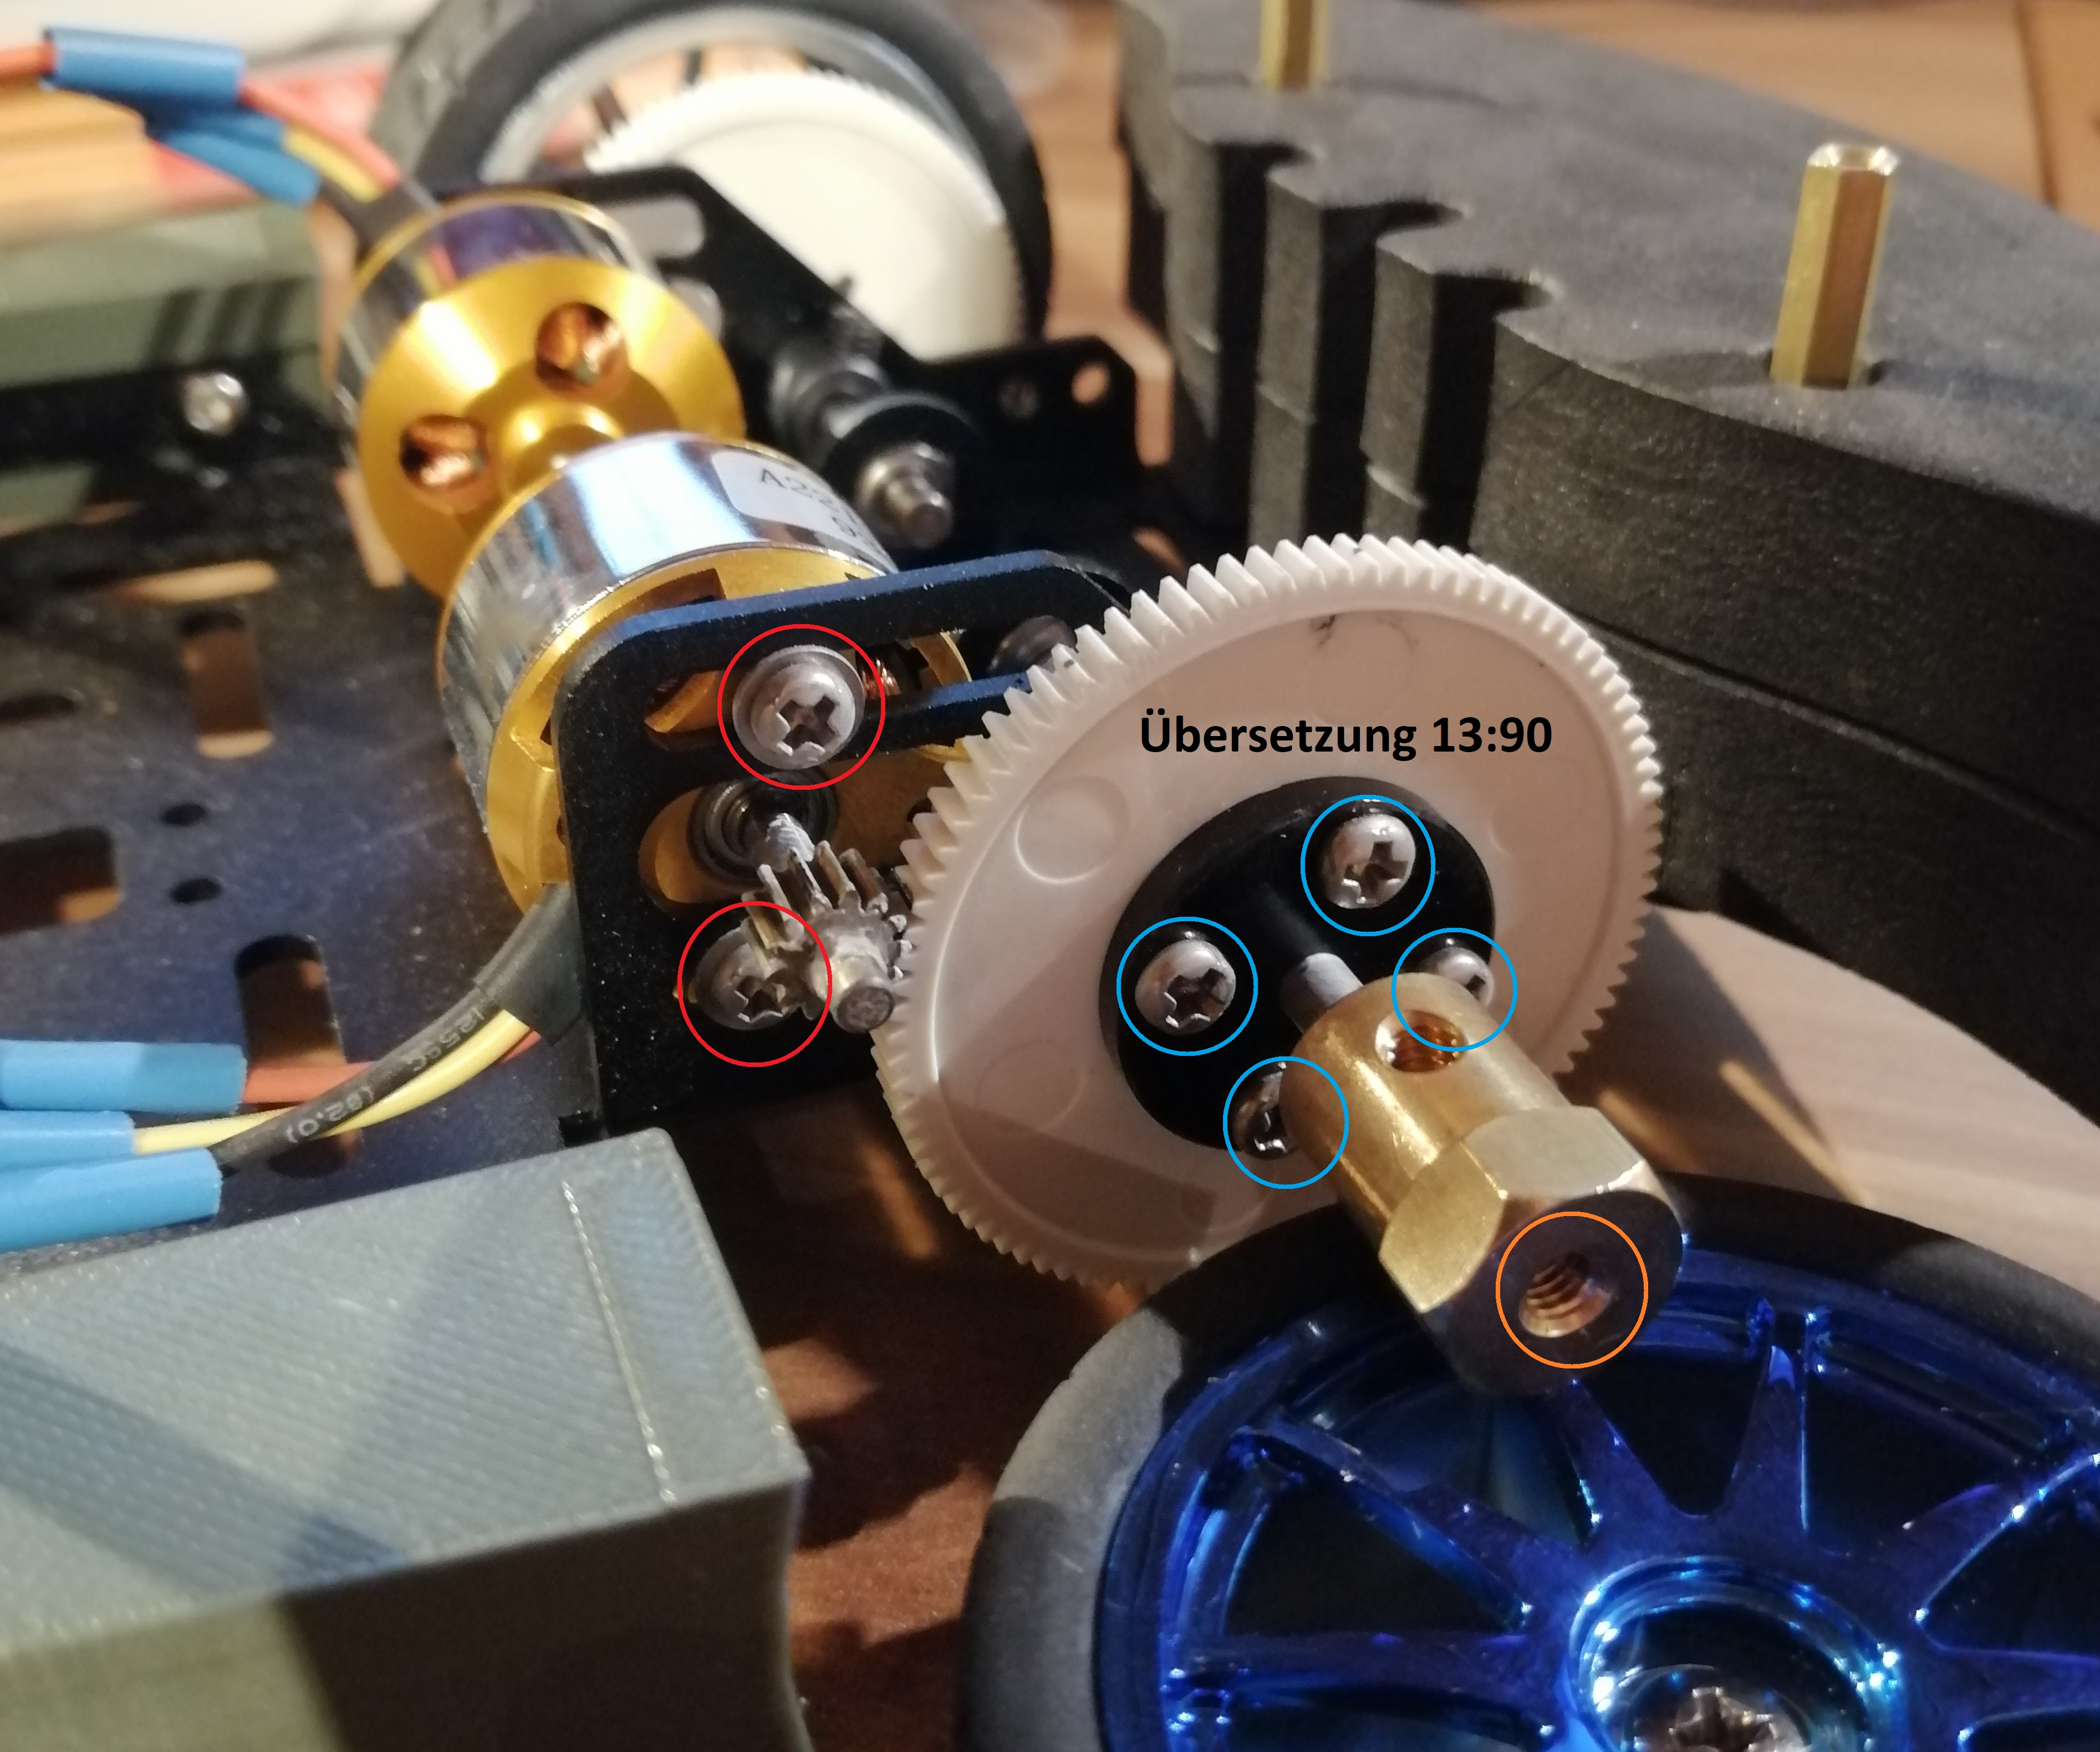
\includegraphics[width=.90\textwidth]{sec4/images/MontageMotorUebersetzung} 
\centering
\captionsetup{width=.95\textwidth}
\caption[Montage der Antriebskomponenten]{Montage der \acp{BLDCMot} und Übersetzung auf die Antriebsachse; In rot die Befestigung des \ac{BLDCMot}s, in blau die Befestigung des Zahnrads an der Antriebswelle und in orange die Befestigung des Reifens}\centering
\label{fig:MontageMotorUebersetzung}
\end{figure}

\subsection{Konfiguration der Motorcontroller}\label{Sec4Sub3}

Die beiden Motorcontroller erwarten nach dem Zuschalten der Spannungsversorgung eine Initialisierungssequenz. Das Power-On-Ereignis wird vom \ac{ESC} mit drei Tönen (tief, mittel, hoch) signalisiert. Im Anschluss daran soll der Wert an der Signalleitung größer als 0\% sein. Das bedeutet, dass ein \ac{PWM}-Signal angelegt werden muss, welches eine Drehzahl N $\geq$ 0rpm repräsentiert. Der \ac{ESC} quittiert das Erkennen des \ac{PWM}-Signals mit einem tiefen Ton. Die Initialisierungssequenz ist allerdings erst dann beendet, wenn das \ac{PWM}-Signal an der Signalleitung zuerst vergrößert und dann auf 0\% verringert wird (N = 0rpm). Dabei gibt der \ac{ESC} einen letzten, hohen Ton von sich. Der Ablauf der Initialisierungssequenz ist in Abbildung \ref{fig:initESC} dargestellt. Nach dem letzten Ton ist die Initialisierung beendet und der \ac{BLDCMot} dreht sich in Abhängigkeit des an der Signalleitung anliegenden \ac{PWM}-Signals. 

\begin{figure}[H] %H für Positionierung hier
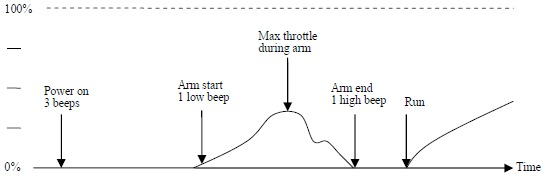
\includegraphics[width=.90\textwidth]{sec4/images/BLDCInit} 
\centering
\captionsetup{width=.95\textwidth}
\caption[Initialisierungssequenz der \ac{ESC}s]{Initialisierungssequenz der \ac{ESC}s; Wert an der Signalleitung für die Initialisierungssequenz über der Zeit; 0\% entspricht dem \ac{PWM}-Tastgrad für den Stillstand und 100\% dem für die maximal erreichbare Drehzahl}\centering
\label{fig:initESC}
\end{figure}

Da die \ac{ESC}s individuell konfiguriert werden können und in der Dokumentation zu wenige Angaben gemacht werden, ist der Tastgrad für die Werte 0\% (Stillstand) und 100\% (maximal erreichbare Drehzahl) unbekannt. Deshalb ist es nicht möglich zu wissen, welche \ac{PWM}-Tastgrade für die Initialisierungssequenz verwendet werden müssen. Über die Konfiguration der \ac{ESC}s können die Grenzen für 0\% und 100\% selbst festgelegt werden. Für das Flashen der Motorcontroller wird die Software \glqq{}BLHeliSuite\grqq{} verwendet. Die Verbindung zwischen den \ac{ESC}s und der Software stellt ein Arduino Nano her.\vspace{11pt}

Der Arduino Nano muss zuvor mit einer neuen Software beschrieben werden. Um die \ac{ESC}s flashen zu können wird der Signalpin des zu programmierenden \ac{ESC} mit dem Pin D3 und der Massepin der Signalleitung mit einem Massepin des Arduino Nano verbunden. Danach wird in der Software \glqq{}BLHeliSuite\grqq{} im Reiter \glqq{}Make Interface\grqq{} eine neue Schnittstelle erstellt (siehe Abbildung \ref{fig:ConfigBLHeliSuite}). Auf der rechten Seite des Programm-Fensters wird ein Arduino Nano als Schnittstelle eingerichtet. Mit einem Klick auf den Button \glqq{}Arduino 4way-interface\grqq{} wird die neue Software, durch die die \ac{ESC}s neu konfiguriert werden können, auf den Arduino Nano geladen.

\begin{figure}[H] %H für Positionierung hier
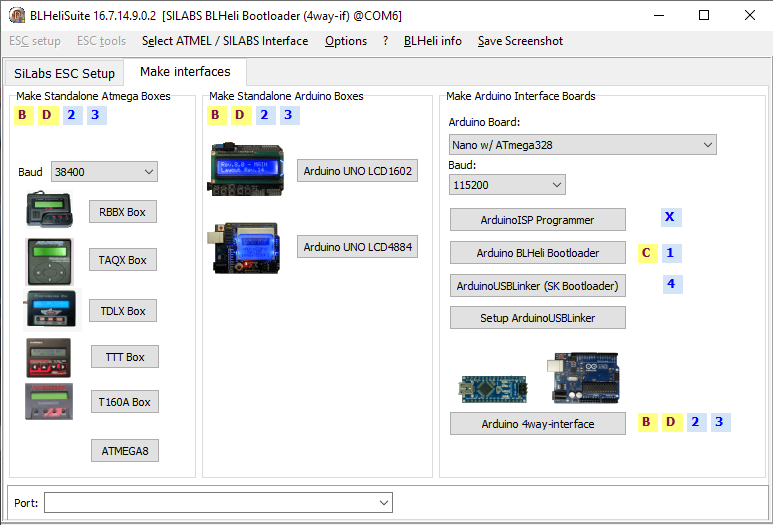
\includegraphics[width=.78\textwidth]{sec4/images/Config_BLHeliSuite} 
\centering
\captionsetup{width=.95\textwidth}
\caption[Programmierung des Arduino Nano zur \ac{ESC}-Konfiguration]{Programmierung des Arduino Nano zur \ac{ESC}-Konfiguration mit der Software BLHeliSuite}\centering
\label{fig:ConfigBLHeliSuite}
\end{figure}

Nach dem Programmieren des Arduino Nano wird die Kommunikation der BLHeliSuite-Software mit dem \ac{ESC} hergestellt. Über die Schaltfläche \glqq{}Read Setup\grqq{} werden die voreingestellten Parameter des \ac{ESC} ausgelesen. Im nächsten Schritt werden die Zeiten für die Werte \glqq{}PPM min Throttle\grqq{} (0\% Aussteuergrad) und \glqq{}PPM max Throttle\grqq{} (100\% Aussteuergrad) auf 1100µs und 1900µs angepasst. Alle vorgenommenen Einstellungen sind in Abbildung \ref{fig:BLHeliSuite} einsehbar. Die Werte werden über die Betätigung der Schaltfläche \glqq{}Write Setup\grqq{} auf den \ac{ESC} geladen. Da jetzt die Werte für 0\% und 100\% Aussteuerung bekannt sind, können die einzelnen Schritte der Initialisierung im Programm des Fahrzeugs abgearbeitet werden.

\begin{figure}[H] %H für Positionierung hier
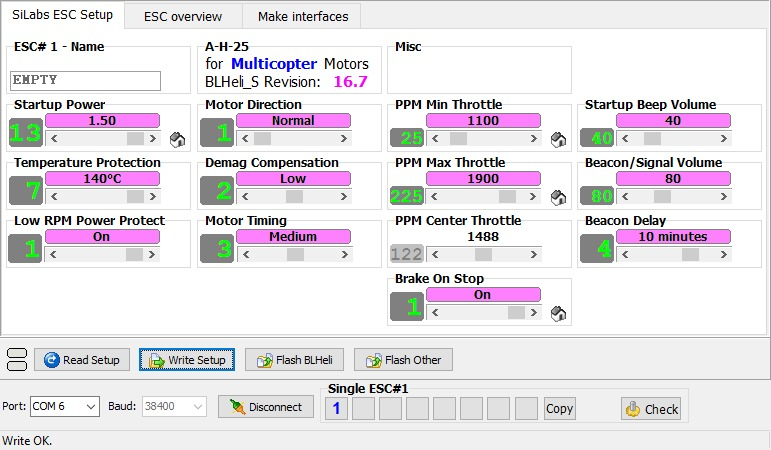
\includegraphics[width=.78\textwidth]{sec4/images/ESC_config} 
\centering
\captionsetup{width=.95\textwidth}
\caption[Parameter der neuen \ac{ESC}-Konfiguration]{Konfiguration der \ac{ESC}s mit der Software \glqq{}BLHeliSuite\grqq{}}\centering
\label{fig:BLHeliSuite}
\end{figure}

\subsection{Programmierung des Antriebsbausteins}\label{Sec4Sub4}

Der Antriebsbaustein der Software ist in zwei Dateien unterteilt, die Dateien \glqq{}drive.c\grqq{} und \glqq{}drive.h\grqq{}. Die Datei \glqq{}drive.h\grqq{} enthält alle relevanten Bibliotheken und Prototypen für die Datei \glqq{}drive.c\grqq{}.\vspace{11pt}

Außer der Einbindung der Bibliotheken und der Prototypen der Funktionen aus der Datei \glqq{}drive.c\grqq{} sind hier auch die Parameter für die Initialisierungssequenz der \ac{ESC}s und für die Initialisierung des Timers für die \ac{PWM}-Signale hinterlegt (Abbildung \ref{fig:DriveH}). 

\begin{figure}[H] %H für Positionierung hier
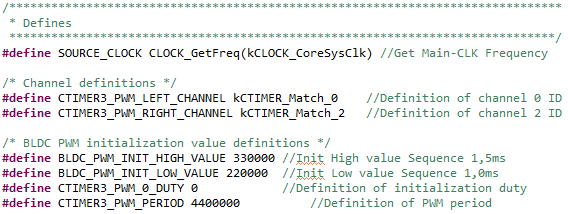
\includegraphics[width=.85\textwidth]{sec4/images/DriveH} 
\centering
\captionsetup{width=.95\textwidth}
\caption[Relevante Zeilen der Datei \glqq{}drive.h\grqq{}]{Relevante Zeilen der Datei \glqq{}drive.h\grqq{} mit den Parametern für die Initialisierungssequenz der \ac{ESC}s und für die Initialisierung des \ac{PWM}-Timers}\centering
\label{fig:DriveH}
\end{figure}

Für die \ac{PWM}-Periodendauer wird bei der Initialisierung ein Wert von 4.400.000 Takten festgesetzt, woraus mit einer \ac{CPU}-Taktfrequenz von 220MHz (220.000.000 Takte pro Sekunde) eine Periodendauer von 20ms resultiert. Die Pulsbreite wird während des Programmablaufs regelmäßig überschrieben.\vspace{11pt}

Der \ac{ESC}-Initialisierungswert für den Stillstand (\glqq{}BLDC\_PWM\_INIT\_LOW\_VALUE\grqq{}, 220.000) entspricht hier einer \ac{PWM}-Pulsbreite von 1,0ms und der Initialisierungswert für die in etwa mittlere Aussteuerung (\glqq{}BLDC\_PWM\_INIT\_HIGH\_VALUE\grqq{}, 330.000) einer Breite von 1,5ms. Die volle Aussteuerung der Motoren wird, wie über die \glqq{}BLHeliSuite\grqq{} festgelegt, bei einer Pulsdauer von 1,9ms erreicht (BLDCMaxValue 1900µs, ca. 418.000). Eine Drehzahl von N = 0rpm wird theoretisch über die bei der \ac{ESC}-Konfiguration festgelegten 1,1ms ermöglicht (242.000). Da das \ac{PWM}-Signal leicht abweicht, wird ein etwas geringerer Wert veranlagt (BLDCMinValue 1090µs, ca. 240.000). Damit wird sichergestellt, dass sich die Räder im Stillstand nicht drehen.\vspace{11pt}

Die Parameter BLDCMaxValue und BLDCMinValue existieren im Code für die linke und rechte Antriebsseite separat (\glqq{}BLDCLeftMaxValue\grqq{}, \glqq{}BLDCLeftMinValue\grqq{} \& \glqq{}BLDCRightMaxValue\grqq{}, \glqq{}BLDCRightMinValue\grqq{}). Die Werte dieser Parameter kommen direkt aus dem \ac{EEPROM} und können mit dem Bedienungsboard eingestellt werden (siehe Abbildung \ref{fig:DriveC0}).\vspace{11pt}

\begin{figure}[H] %H für Positionierung hier
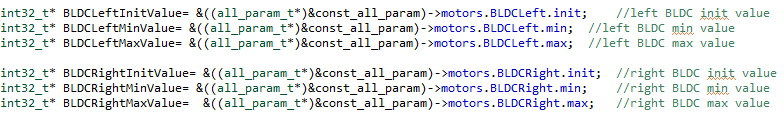
\includegraphics[width=.95\textwidth]{sec4/images/DriveC0} 
\centering
\captionsetup{width=.95\textwidth}
\caption[Extremwerte der Antriebsgeschwindigkeit als Parameter aus dem \ac{EEPROM}]{Extremwerte der Antriebsgeschwindigkeit als Parameter aus dem \ac{EEPROM}, deren Werte über das Bedienungsboard individuell einstellbar sind; Teil der Datei \glqq{}drive.c\grqq{}}\centering
\label{fig:DriveC0}
\end{figure}

\begin{figure}[H] %H für Positionierung hier
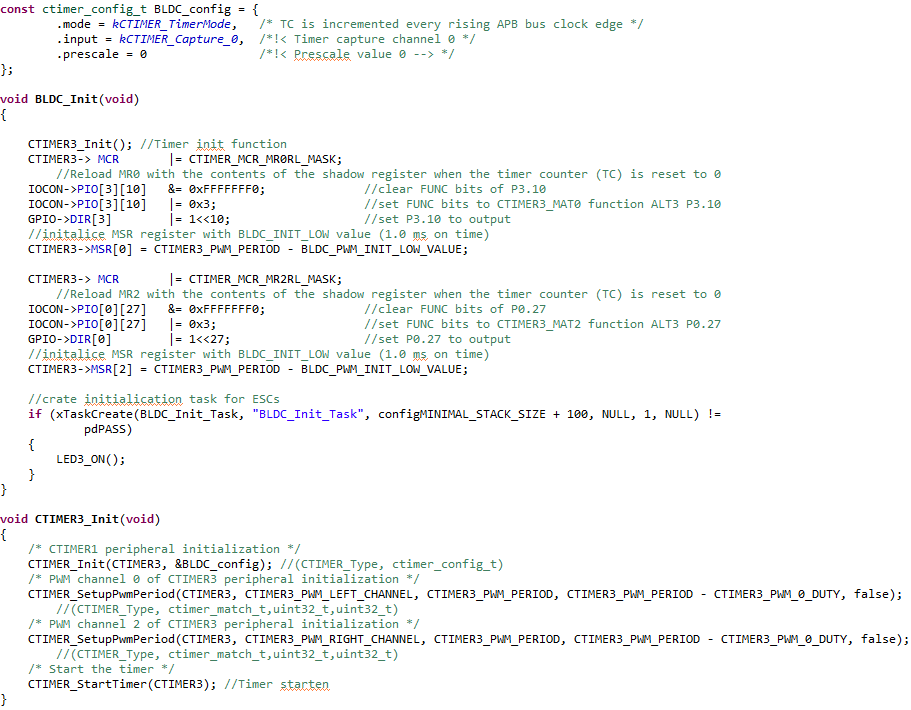
\includegraphics[width=.90\textwidth]{sec4/images/DriveC1} 
\centering
\captionsetup{width=.95\textwidth}
\caption[Funktionen BLDC\_Init und CTIMER3\_Init der Datei \glqq{}drive.c\grqq{}]{Funktionen BLDC\_Init und CTIMER3\_Init der Datei \glqq{}drive.c\grqq{}}\centering
\label{fig:DriveC1}
\end{figure}

Auch die beiden \ac{PWM}-Timer (einer je Motorcontroller) benötigen bei der Initialisierung einige Parameter, deren Werte in der Datei \glqq{}drive.h\grqq{} festgelegt sind (PWM-Periodendauer, \ac{PWM}-Pulsdauer, Kanäle). Die Kanäle werden auf das Timer Match Register 2 (rechter Antrieb, \glqq{}kCTIMER\_Match\_2\grqq{}) und auf das Timer Match Register 0 (linker Antrieb, \glqq{}kCTIMER\_Match\_0\grqq{}) festgelegt, was bei dem verwendeten Controller den Pins P0.27 (rechts) und P3.10 (links) entspricht. Der Pin P3.10 wird auf der Controllerplatine über den Pin 7 und der Pin P0.27 über den Pin 12 der Buchsenleiste J13 nach außen geführt. Der Anschluss der Motorcontroller ist über den Anhang \glqq{}\nameref{SecAtt1}\grqq{} nachvollziehbar.\vspace{11pt}

Die Datei \glqq{}drive.c\grqq{} enthält die Funktionen zur Initialisierung der für die Verwendung der Antriebe notwendigen Controller-Peripherie (siehe Abbildung \ref{fig:DriveC1}) und zur Initialisierung der Motorcontroller (siehe Abbildung \ref{fig:DriveC2}).\vspace{11pt}

In der Funktion BLDC\_Init wird zuerst die Funktion CTIMER3\_Init aufgerufen, welche die beiden vorher festgelegten Kanäle des Timers C3 (\glqq{}kCTIMER\_Match\_0\grqq{} und \glqq{}kCTIMER\_Match\_2\grqq{}) mit den in der Datei ''drive.h'' festgelegten Parametern als \ac{PWM}-Timer mit einer Periodendauer von 20ms und einer Pulsdauer von 0ms initialisiert. Im Anschluss daran wird einzeln für beide Kanäle festgelegt, dass bei einem Timer-Überlauf die neuen Daten für die Pulslängen aus den Shadow-Registern geladen werden sollen. Zum Ändern der Geschwindigkeit eines der beiden Antriebe muss deshalb lediglich ein neuer Wert in das Shadow-Register geschrieben werden. Hier muss allerdings aufgepasst werden, da das Register nicht die Pulsbreite (On-Time) sondern die Off-Time erwartet. Deshalb muss der Wert, der eingetragen wird, der Periodendauer abzüglich der Pulsdauer entsprechen. Zusätzlich werden in der Funktion BLDC\_Init auch die Pins P3.10 und P0.27 für die Verwendung als \ac{PWM}-Ausgang des Timers C konfiguriert. Am Ende wird noch der erste \ac{ESC}-Initialisierungswert in die beiden Shadow-Register geschrieben, bevor die \ac{ESC}-Initialisierungsfunktion aufgerufen wird (siehe Abbildung \ref{fig:DriveC2}).\vspace{11pt}

Der Task BLDC\_Init\_Task beginnt mit dem Befüllen der Shadow-Register mit dem ersten Initialisierungswert. Nach einer Wartezeit von 2s wird der zweite Initialisierungswert in die Register geschrieben. Ebenfalls nach einer Zeit von 2s wird dann wieder der erste Initialisierungswert in die Shadow-Register geschrieben und die Initialisierung der \ac{ESC}s ist abgeschlossen. Die Wartezeiten sind notwendig, damit die \ac{ESC}s Zeit haben, die Änderungen zu erfassen.

\begin{figure}[H] %H für Positionierung hier
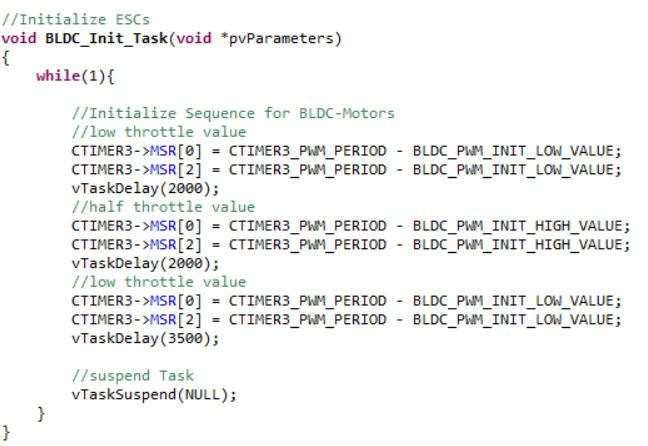
\includegraphics[width=.9\textwidth]{sec4/images/DriveC2} 
\centering
\captionsetup{width=.95\textwidth}
\caption[Funktion BLDC\_Init\_Task der Datei \glqq{}drive.c\grqq{}]{Funktion BLDC\_Init\_Task der Datei \glqq{}drive.c\grqq{} zum Durchlaufen der Initialisierungssequenz der \ac{ESC}s}\centering
\label{fig:DriveC2}
\end{figure}





\newpage
\subsection{Drehzahlmessung}\label{Sec4Sub5}

Im folgenden Abschnitt zur Drehzahlmessung werden deren Notwendigkeit sowie Entwicklungsschritte und Realisierung erarbeitet. Des weiteren wird auch ein Ausblick für die Weiterentwicklung Schaltung gegeben.

\subsubsection{Erörterung der Notwendigkeit einer Drehzahlmessung}\label{Sec:NotwendigkeitDrehzahlmessung}

Die Quellspannung von Akkus verringert sich mit steigender Betriebszeit, weshalb bereits bei vorherigen Fahrzeug-Versionen eine Drehzahlmessung benötigt wird, um über eine Regelung die Spannungsabhängigkeit der Drehzahl bei \acp{DCMot} ausgleichen zu können. Die Spannungsabhängigkeit von \acp{DCMot} bereitet insbesondere beim Überfahren eines Hügels Probleme. Da die in den vorangegangenen Fahrzeugmodellen verwendeten \acp{DCMot} durch \acp{BLDCMot} ersetzt werden, stellt sich allerdings erneut die Frage nach der Notwendigkeit einer Drehzahlmessung. Die Variation der Drehzahl erfolgt bei \acp{DCMot} über die Änderung der Betriebsspannung, was auch die Abhängigkeit von der Versorgungsspannung erklärt. Die Drehzahlvariation bei einem \ac{BLDCMot} wird hingegen über eine Frequenzänderung der Strangspannungen realisiert. Zur Klärung der Frage nach einer Spannungsabhängigkeit der \acp{BLDCMot}, ist eine Messung am Prüfstand erforderlich.

\begin{figure}[H] %H für Positionierung hier
\includegraphics[width=.73\textwidth]{sec4/images/Pruefstand_Messung_UAbhängigkeit} 
\centering
\captionsetup{width=.95\textwidth}
\caption[Messaufbau zur Prüfung der Spannungsabhängigkeit der \acp{BLDCMot}]{Messaufbau zur Prüfung der Spannungsabhängigkeit der \acp{BLDCMot}; in blau die Befestigung des Hecks an der Grundplatte des Prüfstands, in gelb die Befestigung der Vorderreifen am Prüfstand, in rot die DC-Motoren zur Spannungsmessung}\centering
\label{fig:Pruefstand01}
\end{figure}

Für die Durchführung der Messung wird ein bereits vorhandener Prüfstand für Modellfahrzeuge verwendet (siehe Abbildung \ref{fig:Pruefstand01}), welcher im Rahmen einer Bachelor-Abschlussarbeit an der HAW Landshut erstellt worden ist. Damit das Fahrzeug möglichst stabil auf dem Prüfstand steht und die Räder des Fahrzeugs ihre Rotationsbewegung besser auf die \acp{DCMot} des Prüfstands übertragen können, wird das Heck des Fahrzeugs mit Hilfe eines Drahtes am Prüfstand befestigt (Abbildung \ref{fig:Pruefstand01} blaue Markierung). Die vorderen Räder des Fahrzeuges sind ebenfalls am Prüfstand fixiert (Abbildung 44 gelbe Markierungen). \vspace{11pt}

Zur Überprüfung einer eventuellen Abhängigkeit der Drehzahl von der Versorgungsspannung, wird die Spannung an den vorhandenen \acp{DCMot} des Prüfstands gemessen, da diese direkt proportional zur Drehzahl ist (siehe Gleichung \ref{eq4.1}). Die Abhängigkeit der gemessenen Spannung von der Drehzahl ist allerdings nur annähernd linear, da die Drehmomentkonstante k\textsubscript{i} bei hohen Drehzahlen leicht einbricht. Aufgrund der für die Messung konstant eingestellten Pulsbreite von 1,5ms, spielt der Einbruch der Drehmomentkonstante allerdings keine große Rolle, da sich die Drehzahl, wenn überhaupt, nur sehr gering ändert. Dieser Zusammenhang kann deshalb vereinfachend als linear angenommen werden.\vspace{11pt}

Die Versorgungsspannung der \acp{ESC} wird für die Aufnahme verschiedener Messwerte zwischen 6,1V und 8V variiert. Ändert sich die gemessene Spannung mit der Variation der Versorgungsspannung, so ist das ein hinreichender Beweis dafür, dass die Drehzahl der \acp{BLDCMot} spannungsabhängig ist. Die Ergebnisse der Messreihe aus Tabelle \ref{tab:PruefstandMess01} sind zur einfacheren Auswertung in Abbildung \ref{fig:Pruefstand02} visualisiert.

\begin{equation}\label{eq4.1}
U_A = k_i \cdot N \cdot \frac{\pi}{30}
\end{equation}

\begin{table}[H]
\begin{tabular}{|c|c|c|c|c|c|c|c|c|c|c|}
\hline
\rule{0pt}{15pt} Messung & 1&2&3&4&5&6&7&8&9&10 \\
\hline
U\textsubscript{Versorgung} [$V$]&8.0&7.9&7.8&7.7&7.6&7.5&7.4&7.3&7.2&7.1 \\ 
\hline
U\textsubscript{Messung} [$V$]&5.80&5.75&5.65&5.57&5.48&5.40&5.35&5.25&5.18&5.09 \\
\hline
\hline
\rule{0pt}{15pt} Messung & 11&12&13&14&15&16&17&18&19&20 \\
\hline
U\textsubscript{Versorgung} [$V$]&7.0&6.9&6.8&6.7&6.6&6.5&6.4&6.3&6.2&6.1 \\ 
\hline
U\textsubscript{Messung} [$V$]&5.05&4.96&4.87&4.82&4.69&4.73&4.66&4.60&4.50&4.45 \\
\hline
\end{tabular}
\centering
\captionsetup{width=.95\textwidth}
\caption[Messreihe 1: Spannungsabhängigkeit Drehzahl]{Messreihe 1: Messwerte für Überprüfung einer eventuellen Spannungsabhängigkeit der Drehzahl}\centering
\label{tab:PruefstandMess01}
\end{table}

Aus Abbildung \ref{fig:Pruefstand02} kann die Erkenntnis abgeleitet werden, dass die Drehzahl der \acp{BLDCMot}, welche proportional zu der an den \acp{DCMot} gemessenen Ankerspannung U\textsubscript{Messung} ist, bei einem Abfallen der Versorgungsspannung nicht konstant bleibt, denn andernfalls wäre die resultierende Gerade eine Horizontale. Deshalb ist die Drehzahl der \acp{BLDCMot} wie die der \acp{DCMot} abhängig von der Versorgungsspannung.\vspace{11pt}

Die sich aus der Messreihe ergebende Erkenntniss, führt zu dem Entschluss, dass eine Drehzahlregelung nicht nur sinnvoll, sondern auch erforderlich ist. Denn während der Durchfahrt des Parcours wird nicht zu jedem Zeitpunkt die volle Drehzahl benötigt. Folglich hat eine Regelung den Vorteil, dass die vorgegebene Drehzahl auch bei einer fortschreitenden Entladung des Akkus weiterhin aufrecht gehalten werden kann. Wird eine feste Geschwindigkeit vorgegeben, kann die Regelung bei fallender Versorgungsspannung der \acp{ESC} das \ac{PWM}-Signal bis zur Stellgrenze (Pulsbreite = 1,9ms) erhöhen. Erst bei Erreichen der Stellgrenze nimmt die Drehzahl linear mit der Versorgungsspannung ab.

\begin{figure}[H] %H für Positionierung hier
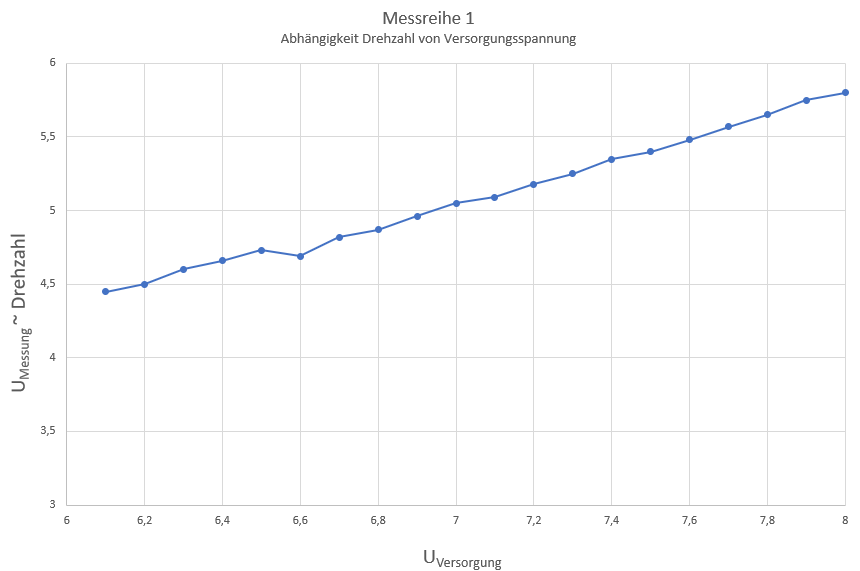
\includegraphics[width=.90\textwidth]{sec4/images/PruefstandMess02} 
\centering
\captionsetup{width=.95\textwidth}
\caption [Spannungsabhängigkeit der Drehzahl von der Versorgungsspannung]{Spannungsabhängigkeit der Drehzahl der \acp{BLDCMot} von der Versorgungsspannung}\centering
\label{fig:Pruefstand02}
\end{figure}

Des weiteren muss das Fahrzeug im Rahmen des NXP-Cups nach dem Überfahren der Ziellinie innerhalb von zwei Metern anhalten können. In der Konfiguration der \acp{ESC} bietet sich dafür die Einstellung \glqq{}Break On Stop\grqq{} an, mit der das Fahrzeug bei einer PWM-Pulsdauer von 1,1ms (BLDCMinValues: BLDCLeftMinValue, BLDCRightMinValue) aktiv bremst, indem die drei Phasen der \acp{BLDCMot} auf Masse geschlossen werden.\vspace{11pt}

Zur Verifizierung eines ordnungsgemäßen Bremsverhaltens, wird eine Probefahrt auf einer langen geraden Strecke an der HAW Landshut durchgeführt. Die Antriebe sind dabei so konfiguriert das sich das Fahrzeug nach der Initialisierung der \acp{BLDCMot} unmittelbar mit maximaler Geschwindigkeit fortbewegt und nach kurzer Fahrtdauer (ca. 3s) stoppt (BLDCMinValues). Hierbei stellt man fest, dass die Bremskraft ausreicht, um das Fahrzeug innerhalb von ca. 30 cm zum Stehen zu bringen.\vspace{11pt}

Während des Testens fällt auf, dass sich die Reifen trotz gleicher ESC-Konfiguration unterschiedlich schnell drehen. Der Grund für dieses Problem lässt darauf schließen, dass die beiden Antriebsseiten einen unterschiedlichen Reibungswert aufweisen. Das kann daran liegen, dass bei den Achsen keine Lager verwendet werden und bei der Übersetzung das Getriebespiel (zwischen den Zahnrädern) auf beiden Antriebsseiten unterschiedlich groß ist, was ebenfalls die Reibung beeinflusst.\vspace{11pt}
%Zum anderen wird davon ausgegangen, dass bei minimalen und maximalen Antrieb die Stellgrenzen (1,09ms und 1,9ms) sprich die ON-Zeit des PWM-Signals kurzfristig über- bzw. unterschritten wird. Befindet sich die Pulsbreite außerhalb des konfigurierten Bereiches schaltet der Antrieb kurzweilig aufgrund des undefinierten Signalzustandes ab und bei Rückkher in den definierten Bereich wieder an.\vspace{11pt} 

Die Spannungsabhängigkeit der \acp{BLDCMot} sowie das unterschiedliche und reibungsabhängige Drehverhalten der beiden Antriebe, machen eine Drehzahlregelung zwingend erforderlich, um ein zuverlässiges und sicheres Fahrverhalten zu gewährleisten.

\subsubsection{Auswahl des Messprinzips}\label{Sec4Sub5Sub2}

Aufgrund der Erkenntnis, dass eine Drehzahlregelung der \acp{BLDCMot} erforderlich ist, gilt es in diesem Abschnitt entsprechende Messprinzipien zur Drehzahlerfassung gegenüberzustellen und die für dieses Projekt sinnvollste Messmethode zu bestimmen.\vspace{11pt}

Die in bisherigen Fahrzeugversionen am häufigsten verwendeten Methoden zur Drehzahlerfassung sind die Verwendung von Hallsensoren oder Lichtschranken (siehe Abbildung \ref{fig:Vorgaengerfahrzeug}). Hallsensoren und Lichtschranken eignen sich hervorragend für eine berührungslose Drehzahlerfassung. Für die Drehzahlmessung mithilfe von Hallsensoren werden kleine Magnete auf der Innenseite der Hinterräder angebracht, welche vom Hallsensor erfasst werden (Abbildung \ref{fig:Vorgaengerfahrzeug}, links). Anhand der Zeit zwischen den Zuständen \glqq{}Magnet vorhanden\grqq{} oder \glqq{}Magnet nicht vorhanden\grqq{} (HIGH/LOW-Signal), kann unter Berücksichtigung der jeweiligen Getriebeübersetzung und Menge der Magnete die Drehzahl der \acp{BLDCMot} bestimmt werden. Die Drehzahlmessung mit einer Lichtschranke funktioniert in der Auswertung genau wie die Messung mit  Hallsensoren, lediglich die Messmittel sind anders (Abbildung \ref{fig:Vorgaengerfahrzeug}, rechts).

\begin{figure}[H] %H für Positionierung hier
\includegraphics[width=.4\textwidth]{sec4/images/Vorgängerfahrzeug} 
\includegraphics[width=.4\textwidth]{sec4/images/Vorgängerfahrzeug_zwei} 
\captionsetup{width=.95\textwidth}
\centering
\caption[Varianten der Drehzahlerfassung bei vorherigen Fahrzeugversionen]{Varianten der Drehzahlerfassung bei vorherigen Fahrzeugversionen; links: Hallsensoren; rechts: Lichtschranke}\centering
\label{fig:Vorgaengerfahrzeug}
\end{figure}     


Ein Hallsensor bietet den Vorteil, dass neben der Erfassung der Drehzahl auch die Drehrichtung mit Hilfe eines zweiten um 90° versetzten Hallsensors bestimmt werden kann. Dazu muss nicht einmal ein zweiter Sensor gekauft werden, da bereits zwei Hallsensoren in einem Gehäuse verbaut sind. Im Zuge dieser Projektarbeit ist eine Erfassung der Drehrichtung jedoch nicht erforderlich, da die für die \acp{BLDCMot} verwendeten \acp{ESC} so konfiguriert sind, dass nur eine Fahrt in Vorwärtsrichtung möglich ist. Ein weiterer Vorteil des Hallsensors aber auch einer Lichtschranke ist, dass die für die GPIO-Pins notwendigen Rechtecksignale direkt vorgegeben werden und keine zusätzliche Umformung des Signals mehr notwendig ist. \vspace{11pt}

Aufgrund der Klebebefestigung der Magnete besteht das Risiko, dass diese sich nach einer gewissen Zeit ablösen und somit die Daten zur Drehzahlerfassung verfälschen. Wie in Abbildung \ref{fig:Vorgaengerfahrzeug} zusätzlich zu erkennen ist, ist die Montage des Hallsensors, die lediglich über die Versorgungsdrähte oder eine zusätzliche Drahtstütze realisiert ist, sehr anfällig auf Erschütterungen. Eine zuverlässige und weniger erschütterungsempfindliche Montage des Hallsensors erfodert deshalb eine zusätzliche Halterung (3D-Druck Anbauteil). Diese Halterung muss erst konstruiert, gedruckt und montiert werden. Um mechanische Probleme, wie sie durch Erschütterungen entstehen können, vollständig zu eliminieren, bietet sich die Anwendung eines anderen, bisher noch nicht erwähnten Messprinzips an, auf welches in weiteren Verlauf genauer eingegangen wird.\vspace{11pt}

Die Alternativmethode zur Erfassung der Drehzahl ist die Anbindung eines Tiefpassfilters mit nachgeschaltetem Komparator an eine der \ac{BLDCMot}-Phasen. Die Schaltung filtert die hochfrequenten Anteile des Phasensignals heraus. Mithilfe einer Komparatorschaltung wird daraus ein Rechtecksignal mit steilen Flanken erzeugt. Hierbei wird das auf der Phase vom \ac{ESC} bereitgestellte, hochfrequente Signal (Abbildung \ref{fig:Signaldarstellung}, grüner Signalverlauf V(in)) abgegriffen. Durch die mit dem Schaltungssimulationstool LTSpice entwickelte und auf einer Lochrasterplatine in Hardware realisierte Tiefpass- und Komparatorschaltung kann dieses abgegriffene Signal in ein eindeutiges Rechtecksignal umgeformt werden (Abbildung \ref{fig:Signaldarstellung}, pinker Signalverlauf V(out)).\vspace{11pt}

Bei der Drehzahlmessung wird der zeitliche Abstand zwischen zwei aufeinanderfolgenden, steigenden Flanken des aus der Tiefpass-/Komparatorschaltung generierten Rechtecksignals mit Hilfe eines Timer-Zählers bestimmt. Die erfassten Zeiten zwischen den Flanken sind proportional zur Drehzahl und können direkt für die Drehzahlregelung verwendet werden, ohne die tatsächliche Drehzahl errechnen zu müssen.\vspace{11pt}

Es gilt zu erwähnen, dass auch bei dieser Methode eine Erfassung der Drehrichtung möglich wäre. Bei drei Phasen, welche um 120° zueinander versetzt sind, kann die Drehrichtung anhand der Pulsreihenfolge der einzelnen Phasen bestimmt werden, wobei nur zwei der drei Phasen benötigt werden. Aufgrund dessen, dass die ESCs lediglich eine feste Drehrichtung erlauben (harte Konfiguration), wird die Drehrichtungsbestimmung nicht benötigt.

\begin{figure}[H] %H für Positionierung hier
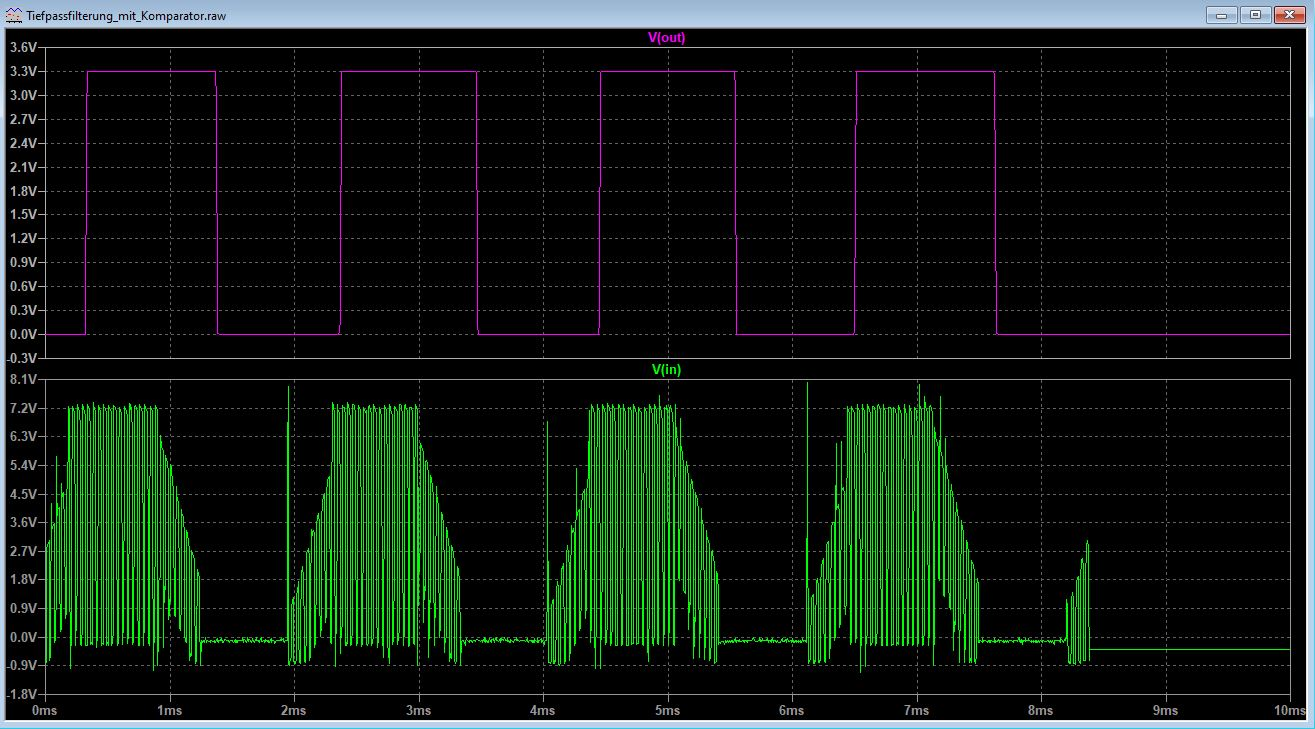
\includegraphics[width=.92\textwidth]{sec4/images/Signaldarstellung} 
\centering
\captionsetup{width=.95\textwidth}
\caption[Phaseneingangssignal und Ausgangssignal der Tiefpass-/Komparatorschaltung]{Phasensignal eines Antriebs (V(in), grün) bei schneller Fahrt und Darstellung des simulierten Ausgangssignals (V(out), pink) aus der Tiefpass-/Komparatorschaltung; erstellt und simuliert mit dem Schaltungssimulationstool LTspice XVII}\centering
\label{fig:Signaldarstellung}
\end{figure}

Da auch bei diesem Messprinzip ein hoher Aufwand (Entwicklungs- und Simulationsaufwand) erforderlich ist, gilt es abzuwägen, welche dieser Methoden am vorteilhaftesten für das Gesamtprojekt ist. Unter Betrachtung der Vor- und Nachteile aller Messprinzipien bietet sich die Tiefpass-/Komparatorschaltung am meisten an. Insbesondere die Unempfindlichkeit gegen Erschütterungen und die Verwendung der ohnehin von den ESCs bereitgestellten Phasensignale, spricht für die Realisierung der Drehzahlmessung mit dieser Methode. Als weitere Gründe gegen die sonstigen Messprinzipien sprechen die unzuverlässige Montage von Hallsensoren oder Lichtschranken und die fehlende Notwendigkeit einer Erfassung der Drehrichtung.

\newpage

\subsubsection{Hardware für die Drehzahlmessung}\label{Sec4Sub5Sub3}

In diesem Abschnitt wird die Entwicklung der Schaltung zur Drehzahlmessung beschrieben. Dabei wird sowohl auf die Probleme eingegangen, die sich während der Schaltungsentwicklung ergeben als auch auf deren Behebung. Damit das Phasensignal in ein eindeutiges Rechtecksignalsignal umgesetzt werden kann, bedarf es der im vorherigen Abschnitt erörterten Entwicklung einer Tiefpass-/ Komparatorschaltung. Es soll deutlich gemacht werden, welche Bauteile verwendet werden und welchen Zweck diese in der Schaltung erfüllen. Zur Entwicklung und Simulation der Drehzahl-Messschaltung wird das Schaltungssimulationstool LTspice XVII und zur Erstellung des Platinenlayouts die Freeware BlackBoard Circuit Designer verwendet.\vspace{11pt}

Zu Beginn wird die Schaltung für ein Phasensignal in LTspice realisiert. Der daraus resultierende Schaltplan zur Drehzahlmessung ist in Abbildung \ref{fig:Schaltungsaufbau} sichtbar und dient als Überblick über die verwendeten Bauteile mit deren entsprechenden Kennwerten. Es gilt zu erwähnen, dass der Spannungsteiler (R5, R6, R7, R8) zwischen Vref und dem invertierenden Operationsverstärkereingang IN- nur einmal realisiert werden muss, worauf im weiteren noch detaillierter eingegangen wird.

\begin{figure}[H] %H für Positionierung hier
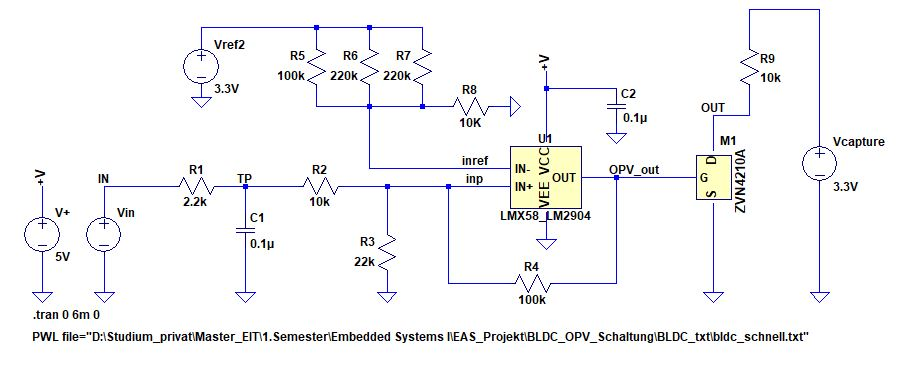
\includegraphics[width=.95\textwidth]{sec4/images/Schaltungsaufbau} 
\centering
\captionsetup{width=.95\textwidth}
\caption[Schaltplan der Tiefpass-/Komparatorschaltung aus LTspice XVII]{Schaltplan der Tiefpass-/Komparatorschaltung; erstellt für die Simulation eines Phasensignals in LTspice XVII}\centering
\label{fig:Schaltungsaufbau}
\end{figure}

Das Phasensignal wird von der Spannungsquelle Vin repräsentiert. Die Signale werden vor der Schaltungsentwicklung zwischen einer Phase eines ESCs und dem Massepotential mit dem Oszilloskop gemessen. Hierzu werden die Antriebe auf den Modell-Prüfstand gestellt und je einmal mit hoher und geringer Drehzahl angesteuert. Es gilt zu erwähnen, dass die erfassten Signale für schnelle und langsame Fahrt nicht den maximalen und minimalen Drehzahlen entsprechen. Das Oszilloskop (DSO-X 3034A) bietet die Möglichkeit die gemessenen Ausgangssignale als .csv-Datei auf einem USB-Stick zu speichern. Das gespeicherte .csv-Datei wird daraufhin als \ac{PWLFile} importiert und einer Spannungsquelle übergeben (rechter Mausklick auf Spannungsquelle / PWL-File anwählen / Pfad .csv-Datei wählen). Bevor die .csv-Datei importiert werden kann, muss die Datei umformatiert werden.\vspace{11pt}

Das ungefilterte Phasensignal besitzt eine Frequenz von ca. 23 kHz. Um die hohen Frequenzanteile des Signals im ersten Schritt zu filtern, wird zunächst ein Tiefpass erster Ordnung benötigt. Die Dimensionierung des Tiefpasses erfolgt mit einem 1,1kOhm Widerstand (R1) und einem 100nF Kondensator (C1). Dabei beträgt die Grenzfrequenz f\textsubscript{G} des Tiefpasses nach Gleichung \ref{eq4.2} 723Hz. Der aus der Simulation resultierende Spannungsverlauf sowie der am Oszilloskop gemessene Spannungsverlauf nach der Tiefpassfilterung sind in den Abbildungen \ref{fig:SpannungsverlaufTPSpice} und \ref{fig:SpannungsverlaufTPReal} dargestellt (unterschiedliche Drehzahlen!).

\begin{equation}\label{eq4.2}
f_G = \frac{ 1 }{2 \cdot \pi \cdot R1\cdot C1 }
\end{equation}

\begin{figure}[H] %H für Positionierung hier
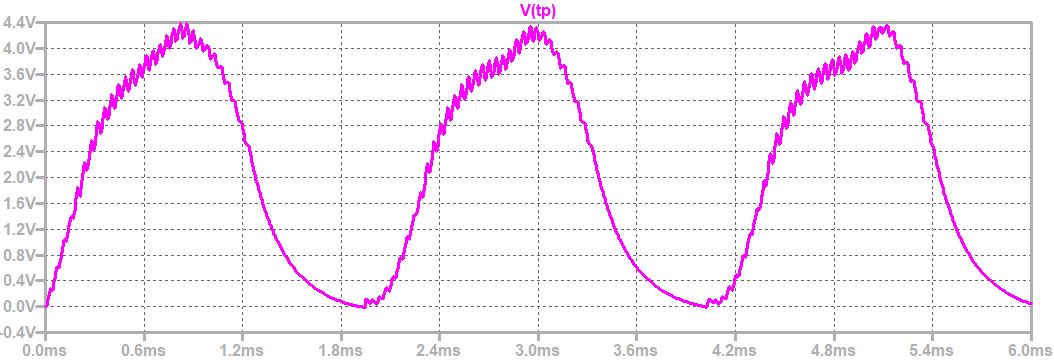
\includegraphics[width=.82\textwidth]{sec4/images/Spannungsverlauf_TP} 
\centering
\captionsetup{width=.95\textwidth}
\caption[Simulationsergebnis des Phasensignals nach dessen Tiefpassfilterung]{Simulationsergebnis des Phasensignals nach dessen Tiefpassfilterung bei schneller Fahrt}\centering
\label{fig:SpannungsverlaufTPSpice}
\end{figure}

\begin{figure}[H] %H für Positionierung hier
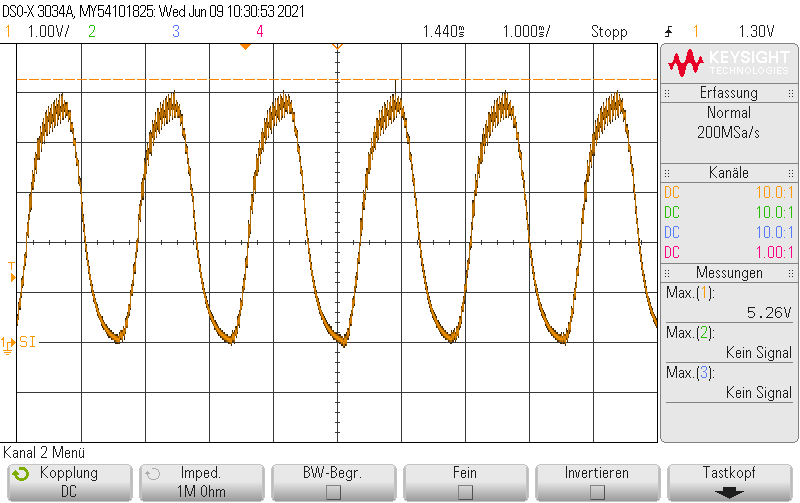
\includegraphics[width=.75\textwidth]{sec4/images/TP} 
\centering
\captionsetup{width=.95\textwidth}
\caption[Messergebnis des Phasensignals nach dessen Tiefpassfilterung]{Messergebnis des Phasensignals nach dessen Tiefpassfilterung bei schneller Fahrt}\centering
\label{fig:SpannungsverlaufTPReal}
\end{figure}

Das zentrale Bauelement der Schaltung ist ein von \ac{TI} hergestellter Operationsverstärker LM358A, welcher als Komparator verwendet wird. Für eine maximal realistische Simulation wird ein Simulations-Modell des Herstellers in LTspice XVII eingebunden \cite{OPVModel}. Hierbei handelt sich um einen \ac{OPV}, welcher im Single-Supply betrieben wird. Der \ac{OPV} wird zunächst mit einer Versorgungsspannung V+ von 5V betrieben, welche wie die Versorgungsspannung des Controllers vom Linearspannungsregler abgegriffen wird. Für die Drehzahlmessung wird jeweils eine Schaltung für das Phasensignal des linken und rechten Antriebs benötigt. Der \ac{OPV} ermöglicht es, beide Signale in einem Bauteil zu verarbeiten. Dazu besitzt er zwei invertierende Eingänge (IN1-, IN2-) und zwei nicht-invertierende Eingänge (IN1+, IN2+) sowie zwei Ausgänge (OUT1, OUT2) (siehe Abbildung \ref{fig:OPVPinbelegung}). Dadurch kann auf der Verteilerplatine zusätzlicher Platz eingespart werden.

\begin{figure}[H] %H für Positionierung hier
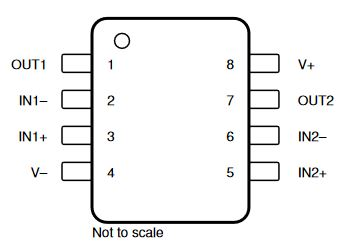
\includegraphics[width=.45\textwidth]{sec4/images/OPV_Pinbelegung} 
\centering
\captionsetup{width=.95\textwidth}
\caption[Pinbelegung des Operationsverstärkers LM358A]{Pinbelegung des Operationsverstärkers LM358A}\centering
\label{fig:OPVPinbelegung}
\end{figure}


Da der \ac{OPV} in der Schaltung als Schmitt-Trigger verwendet wird, müssen einige schaltungstechnische Maßnahmen, wie z.B. ein Spannungsteiler mit Rückführwiderstand hinzugefügt werden. Die Realisierung des Spannungsteilers erfolgt mit den Widerständen R2 = 10kOhm, R3 = 22 kOhm sowie einem Rückführwiderstand R4 = 100kOhm.\vspace{11pt}

Grundsätzlich verstärkt ein \ac{OPV} ständig die Differenz seiner Eingangsgrößen (IN+, IN-). Da ein Operationsverstärker einen theoretisch unendlichen Verstärkungsfaktor besitzt, reicht eine geringe Eingangsspannungsdifferenz aus, um den Ausgang bei dieser Schmitt-Trigger Schaltung in die Versorgungsspannungsbegrenzung zu treiben (nur Werte bis V+). Der verwendete OPV LM358A besitzt einen \glqq{}open-loop voltage gain\grqq{} von 100V/mV. Die Hysterese wird durch den Rückkopplungsanteil (R4) der Ausgangsspannung des \ac{OPV} bestimmt. Aus dieser Art der Rückführung entsteht eine Schmitt-Triggerschaltung welche den Vorteil hat, dass sie unempfindlich gegen Schwankungen innerhalb des Hysteresebandes ist (Schwankungen wie z.B. Rauschen). So wird ein unregelmäßiges Schaltverhalten am \ac{OPV}-Ausgang verhindert und ein sauberes Ausgangssignal erzeugt (siehe Abbildung \ref{fig:inpInrefOpvOut}).\vspace{11pt}

Wie bereits erwähnt kann der Ausgang des OPV im Idealfall seine Versorgungsspannung V+ und V- annehmen. Da das verwendete OPV-Modell nicht über einen Rail-to-Rail Ausgang verfügt, bleibt die maximale Ausgangsspannung stets mit einem nicht zu vernachlässigbarem Abstand unter der Versorgungsspannung. Bei einer \ac{OPV}-Versorgungsspannung V+ von 3,3V werden am Ausgang des OPV ungefähr 2V gemessen. Dies führt dazu, dass das Phasensignal im unteren und oberen Drehzahlbereich die Referenzspannung Vref von 540mV am invertierenden Eingang des OPV nicht durchschreitet. Dadurch wird am OPV-Ausgang kein Rechtecksignal mehr erzeugt. Darüber hinaus ist im zugehörigen Datenblatt des verwendeten Mikrocontrollers ersichtlich, dass die Capture Input Pins vom Timer Modul CTIMER2 (J13 Pin4 / Port-Pin P0.25 für Messung rechts, J13 Pin6 / Port-Pin P0.24 Messung links) eine Mindestspannung von 2,0V benötigten, um zuverlässig einen HIGH-Pegel erkennen zu können. Da dieser Spannungswert insbesondere im niedrigen Drehzahlbereich nie erreicht wird, muss die Versorgungsspannung des OPV hochgesetzt werden. In Abbildung \ref{fig:inpInrefOpvOut} wird die Abweichung bei einer Versorgungsspannung von 5V deutlich. Das Ausgangssignal des Operationsverstärkers (Abbildung \ref{fig:inpInrefOpvOut}, gelb) erreicht einen Spannungspegel von 3.85V. Durch die Erhöhung der Versorgungsspannung kann also grundsätzlich eine höhere Ausgangsspannung erzielt werden.

\begin{figure}[H] %H für Positionierung hier
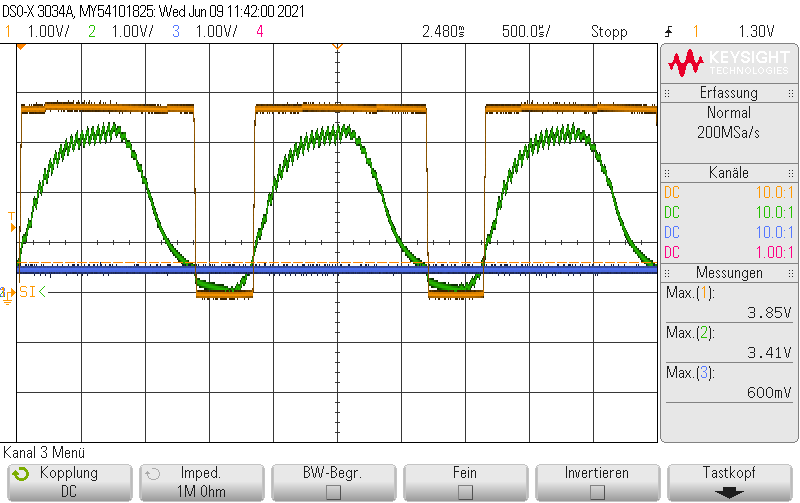
\includegraphics[width=.95\textwidth]{sec4/images/inp_inref_opv_out} 
\centering
\captionsetup{width=.95\textwidth}
\caption[Beispielhafte Messung des OPV-Ausgangssignals bei V+ = 5,0V;]{Beispielhafte Messung des OPV-Ausgangssignals (gelb) bei einer Versorgungsspannung von V+ = 5,0V;  IN+ in grün und Vref an IN- in blau}\centering
\label{fig:inpInrefOpvOut}
\end{figure}

Damit eine Signalspannung mit mehr als 2,0 V für die Capture Input Pins des Timer Moduls CTIMER2 am Mikrocontroller zuverlässig bereit gestellt wird, wird ein n-Kanal MOSFET (ZVN4210A) an jedem der OPV-Ausgänge platziert. Der Widerstand R9 = 10 kOhm vor dem Drain-Anschluss des MOSFETs in Abbildung \ref{fig:Schaltungsaufbau} steht stellvertretend für den internen Pull-up Widerstand der TIMER2 Capture Input Pins des Mikrocontrollers. Je nach Konfiguration können diese zu- oder abgeschalten werden.\vspace{11pt}

Für die Bereitstellung der am invertierenden OPV-Eingang (IN-) benötigten Referenzspannung, auch Schwellspannung genannt, wird ein Spannungsteiler mit einer vom Pin12 der Buchsenleiste J10 stammenden +3,3V Spannungsversorgung vorgeschalten. Der Spannungsteiler besteht aus drei parallel geschaltenen Widerständen R5 = 100kOhm und R6 = R7 = 220kOhm in Reihe zum Widerstand R8 = 10kOhm. Die dadurch erzeugte Referenzspannung beträgt etwa 540mV. Diese Referenzspannung ist in der Theorie ausreichend, um für alle Drehzahlen ein zuverlässiges Rechtecksignal zu erzeugen. Trotz aller bisher getroffenen Optimierungen treten dennoch immer wieder Probleme bei der Drehzahlmessung auf. Die Problematik sowie deren Lösung werden im Kapitel \ref{Sec4Sub5Sub4} \nameref{Sec4Sub5Sub4} beschrieben.

\begin{figure}[H] %H für Positionierung hier
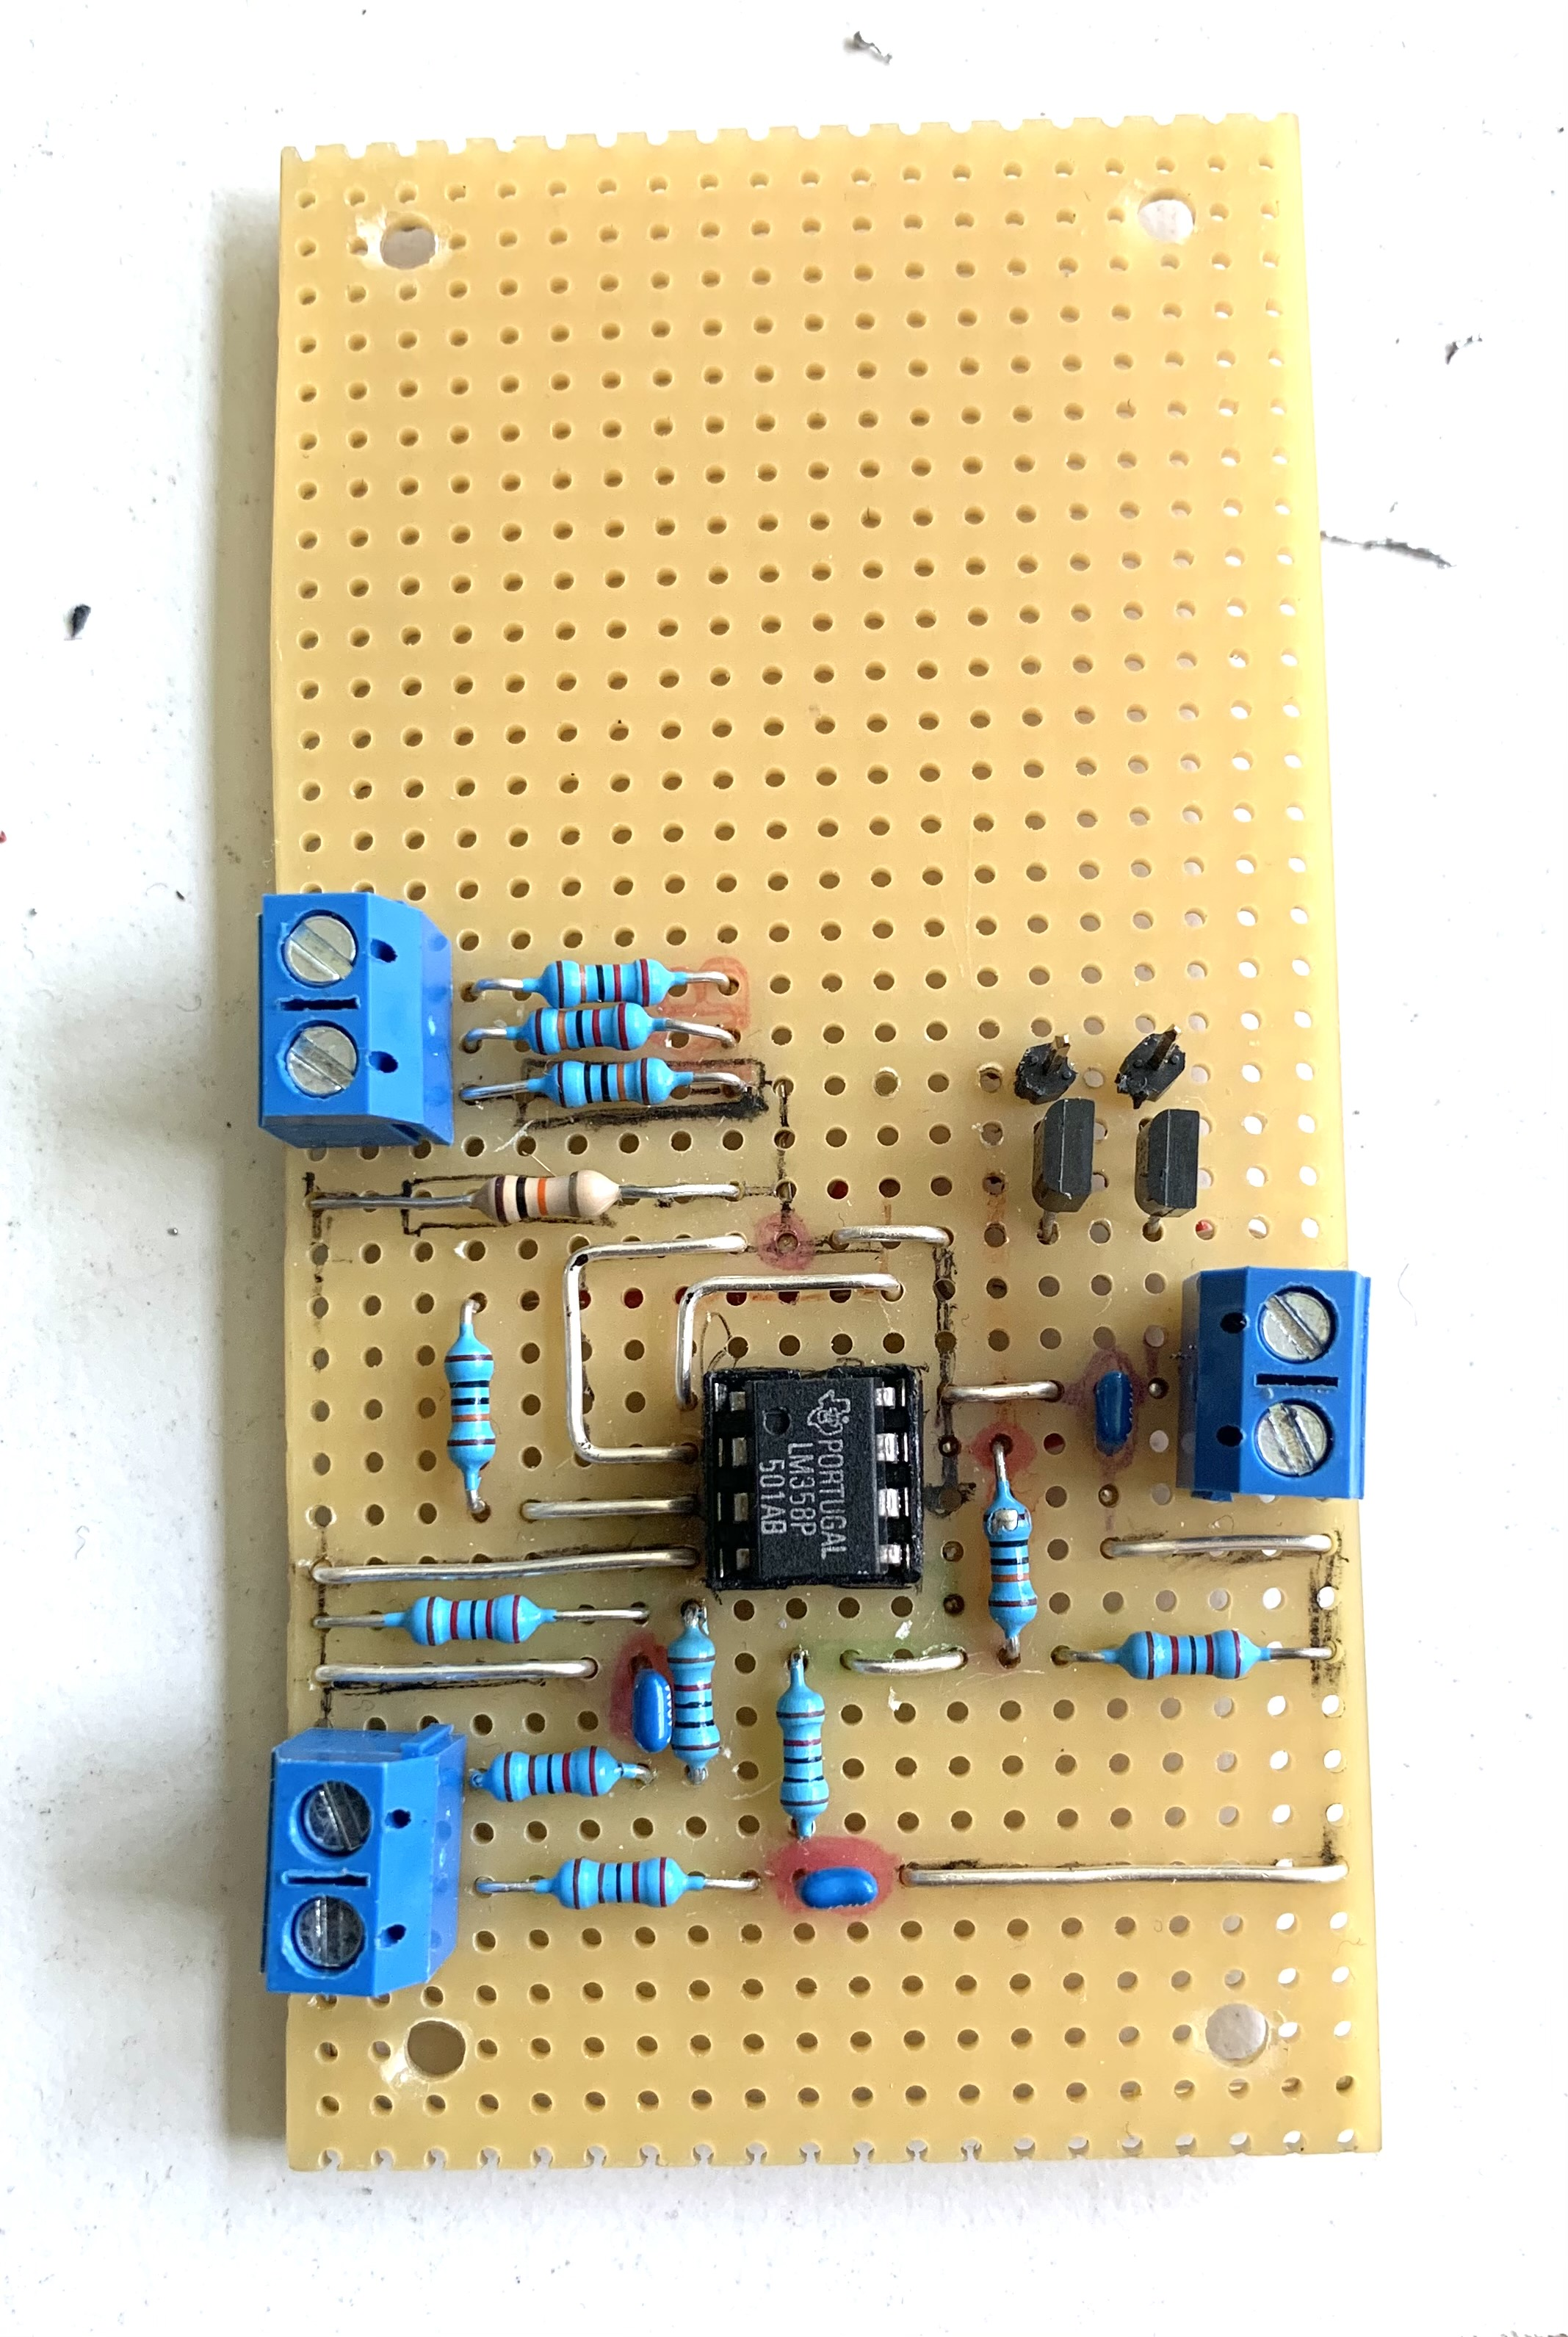
\includegraphics[width=.40\textwidth]{sec4/images/Platine} 
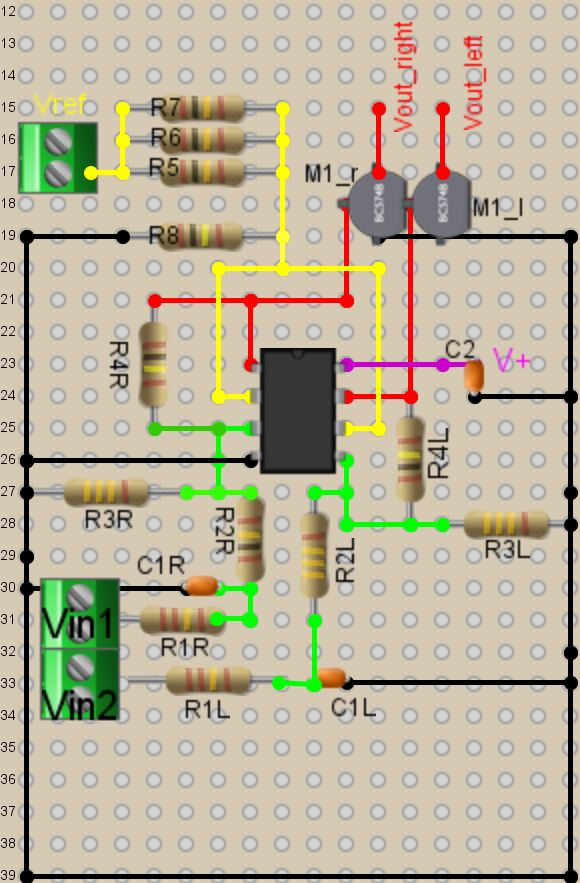
\includegraphics[width=.40\textwidth]{sec4/images/Platinendesign}
\captionsetup{width=.95\textwidth}
\centering
\caption[Schaltung der Drehzahlmessung und zugehöriges Layout] {Schaltung der Drehzahlmessung auf der Signalverteilerplatine (links) und zugehöriges Layout (rechts)}\centering
\label{fig:DrehzahlmessSignalvertPlat}
\end{figure}

Auf der linken Seite der Abbildung \ref{fig:DrehzahlmessSignalvertPlat} ist die auf der Signalverteilerplatine befindliche Drehzahl-Messschaltung im Original zu sehen. Auf der rechten Seite der Abbildung \ref{fig:DrehzahlmessSignalvertPlat} befindet sich das dafür mit dem Programm BlackBoard Circuit Designer erstellte, zugehörige Layout. Die grünen Verbindungen stellen die Pfade zwischen Vin (Phasensignale) und den OPV Eingängen IN1+ und IN2+ dar. Gelbe Linien repräsentieren den Pfad der Referenzspannung Vref zu den invertierenden Eingängen IN1- und IN2-. Der Pfad zur Spannungsversorgung des OPV (V+) ist in violett dargestellt und alle schwarzen Verbindungen stellen GND-Verbindungen dar. Zuletzt kann der Verlauf der Ausgangsspannungen vom OPV an die Capture Eingänge des Timers CTIMER2 anhand der roten Verbindungen nachvollzogen werden. 


\newpage
\subsubsection{Programmierung des Drehzahlmessungsbausteins}\label{Sec4Sub5Sub5}

Damit die durch die Schaltung bereitgestellten Rechtecksignale (links, rechts) vom Mikrocontroller erfasst werden können, werden die Capture Register des Timer-Moduls CTIMER2 verwendet. Dieses Modul löst bei einem Flanken-Ereignis (steigende Flanke) am jeweiligen Capture Input Pin einen Interrupt aus, in welchem die verstrichene Zeit seit der letzten steigenden Flanke errechnet wird und speichert dann den aktuellen Timerwert ab.\vspace{11pt}

Der Softwarebaustein zur Drehzahlerfassung ist in zwei Dateien unterteilt, die Dateien \glqq{}rpmMeas.c\grqq{} und \glqq{}rpmMeas.h\grqq{}. Die Datei \glqq{}rpmMeas.h\grqq{} enthält alle relevanten Bibliotheken und Prototypen für die Datei \glqq{}rpmMeas.c\grqq{} (siehe Abbildung \ref{fig:rpmMeasH}). Hier werden auch die beiden Kanäle zur Erfassung der Daten auf das Timer Caputure Register 0 (rechter Antrieb, \glqq{}kCTIMER\_Capture\_0\grqq{}) und auf das Timer Capture Register 1 (linker Antrieb, \glqq{}kCTIMER\_Capture\_1\grqq{}) festgelegt. Bei dem verwendeten Mikrocontroller entspricht dies den Pins P0.25 (rechts) und P0.24 (links). Der Pin P0.25 wird auf der Controllerplatine über den Pin4 und der Pin P0.24 über den Pin6 der Buchsenleiste J13 nach außen geführt.\vspace{11pt}

\begin{figure}[H] %H für Positionierung hier
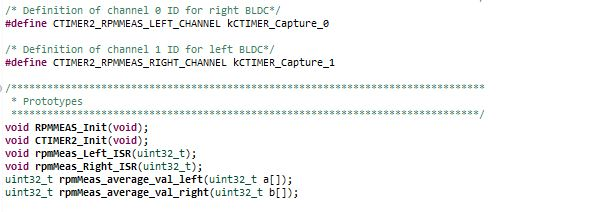
\includegraphics[width=.80\textwidth]{sec4/images/rpm_defines} 
\centering
\captionsetup{width=.95\textwidth}
\caption[Relevante Zeilen der Datei \glqq{}rpmMeas.h\grqq{}]{Relevante Zeilen der Datei \glqq{}rpmMeas.h\grqq{} zur Initialisierung des Timers CTIMER2 für die Zeiterfassung zwischen zwei Flanken Signal sowie die Prototypen für die Funktionen aus der Datei \glqq{}rpmMeas.c\grqq{}}\centering
\label{fig:rpmMeasH}
\end{figure}

Die Datei \glqq{}rpmMeas.c\grqq{} enthält die Funktionen zur Initialisierung der für die Verwendung der Drehzahlerfassung notwendigen Controller-Peripherie als auch die Definition und Initialisierungen der notwendigen Parameter zur Erfassung und Berechnung der benötigten Drehzahlwerte (siehe Abbildung \ref{fig:rpmMeasC0}).\vspace{11pt}

In der Funktion RPMMEAS\_Init wird zuerst die Funktion CTIMER2\_Init aufgerufen, welche unter anderem die beiden vorher festgelegten Kanäle des Timers CTIMER2 (\glqq{}kCTIMER\_Capture\_0\grqq{} und \glqq{}kCTIMER\_Capture\_1\grqq{}) initialisiert. Bei der Initialisierung der Capture Channel (CTIMER\_SetupCapture) wird das entsprechende Ereignis, bei dem ein Capture stattfinden soll, festgelegt. In diesem Fall wird dises Ereignis für beide Kanäle auf die steigende Flanke gesetzt und die Capture Interrupt Requests aktiviert (\glqq{}kCTIMER\_Capture\_RiseEdge\grqq{}).

\begin{figure}[H] %H für Positionierung hier
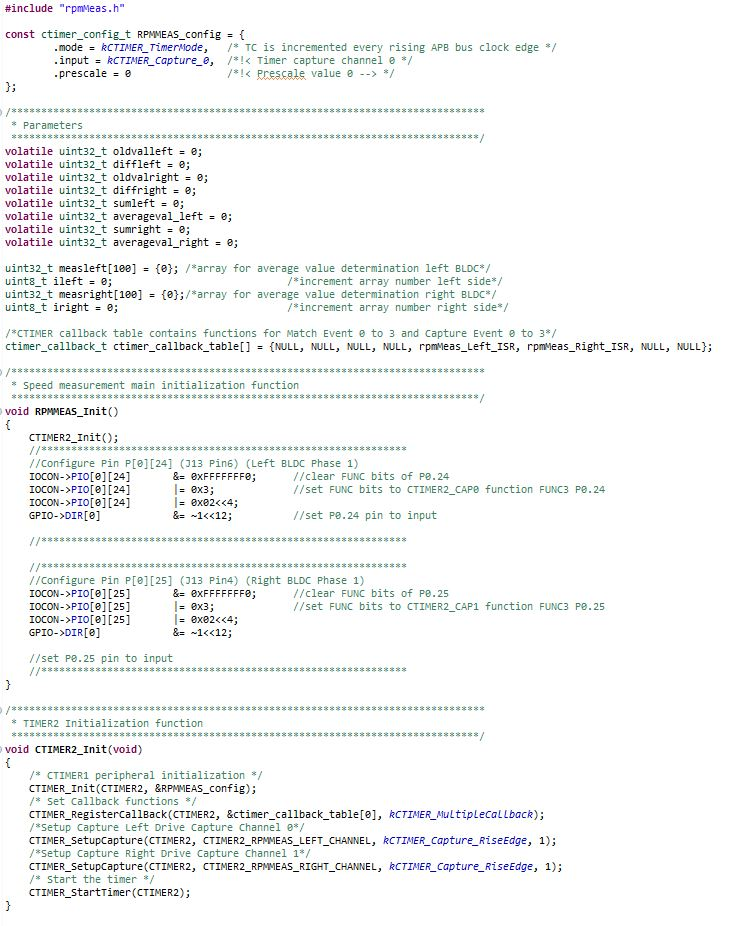
\includegraphics[width=.90\textwidth]{sec4/images/rpmmeas_init_ctimer2_init} 
\centering
\captionsetup{width=.95\textwidth}
\caption[Funktionen RPMMEAS\_Init und CTIMER2\_Init in der Datei \glqq{}rpmMeas.c\grqq{}]{Funktionen RPMMEAS\_Init und CTIMER2\_Init in der Datei \glqq{}rpmMeas.c\grqq{}}\centering
\label{fig:rpmMeasC0}
\end{figure}

Damit beim Auftreten einer steigenden Flanke der Rechtecksignale ein Interrupt Request ausgelöst werden kann, benötigt man zunächst den Parameter cTimer\_callback\_table. Die Callback-Table enthält die bei verschiedenen Events (Match0-3 und Capture0-3) aufzurufenden Interrupt Service Routinen rpmMeas\_Left\_ISR (Capture Event 0) und rpmMeas\_Right\_ISR (Capture Event 1). Die Callback-Table wird als Pointer-Array der Funktion CTIMER\_RegisterCallBack übergeben. Bei einer Callback-Funktion, auch Rückruffunktion genannt, wird einer Funktion als Parameter eine weitere Funktion oder wie hier eine Liste von Funktionen übergeben. Des weiteren muss in der RegisterCallBack-Funktion der Typ des Callbacks festgelegt werden. In diesem Fall wird der Callback als \glqq{}kCTIMER\_MultipleCallback\grqq{} festgelegt, was bedeutet, dass pro Kanal ein Callback durchgeführt werden kann. Zuletzt wird in der CTIMER2\_Init der Timer CTIMER2 gestartet.\vspace{11pt}

Nach Vollendung der Initialisierungen in der Funktion CTIMER2\_Init werden in der Funktion RPMMEAS\_Init zusätzlich die Pins P0.24 (Messung links) und P0.25 (Messung rechts) für die Verwendung als Capture Input Pin des Timers CTIMER2 konfiguriert.\vspace{11pt}

Zur Erfassung der Drehzahl wird im Programm eine Interrupt Service Routine rpmMeas\_Left\_ISR und rpmMeas\_Right\_ISR für die jeweilige Antriebsseite benötigt. Sobald auf eine steigende Flanke getriggert wird, wird durch das Setzen eines Interrupt Flags die Interrupt Service Routine ausgelöst. In der jeweiligen Service Routine wird der aktuelle Zähler-Wert des Timers CTIMER2 mit dem Befehl CTIMER\_GetTimerCountValue ausgelesen, der Wert bei der letzten Flanke abgezogen und somit die verstrichene Zeit zwischen diesen Flanken berechnet (diffright und diffleft) und den Arrays zur Mittelwertberechnung (measright[ ], measleft[ ]) übergeben.  

\begin{figure}[H] %H für Positionierung hier
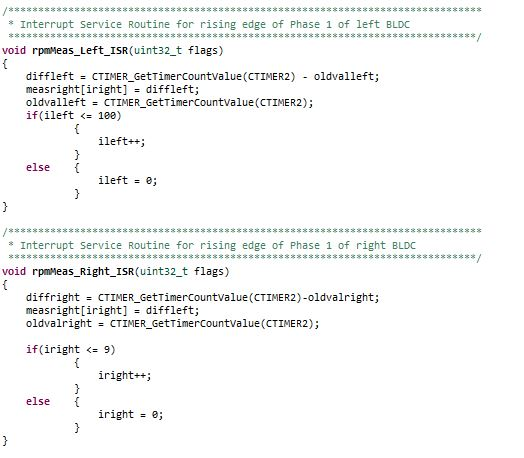
\includegraphics[width=.8\textwidth]{sec4/images/isr} 
\centering
\captionsetup{width=.95\textwidth}
\caption[Interrupt Service Routinen für Zeitermittlung zwischen zwei Capture-Flanken]{Interrupt Service Routinen für Zeitermittlung zwischen zwei Flanken der Capture Inputs des Timers CTIMER2}\centering
\label{fig:isr}
\end{figure}

\newpage
Von den in den Arrays (\glqq{}measright[ ]\grqq{} und \glqq{}measleft[ ]\grqq{}) gespeicherten Werten können in den Funktionen \glqq{}rpmMeas\_average\_val\_right()\grqq{} und \glqq{}rpmMeas\_average\_val\_right()\grqq{} die Mittelwerte gebildet werden. Die Mittelwerte \glqq{}average\_val\_right\grqq{} und \glqq{}average\_val\_left\grqq{} werden in den weiteren Schritten zur Implementierung der Drehzahlregelung benötigt. 

\begin{figure}[H] %H für Positionierung hier
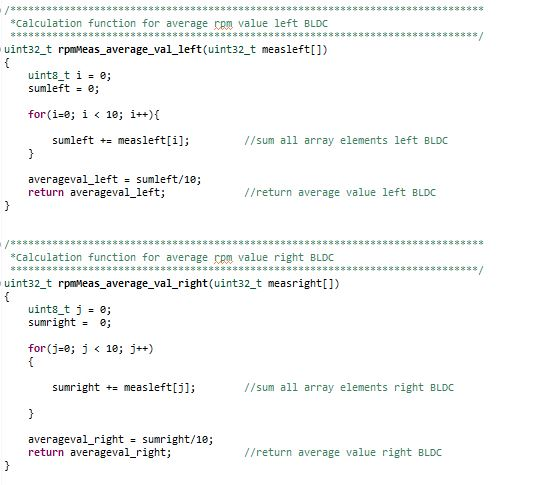
\includegraphics[width=.8\textwidth]{sec4/images/calculation} 
\centering
\captionsetup{width=.95\textwidth}
\caption[Funktionen zur Berechnung des Mittelwerts der Zeiten zwischen den Capture-Flanken]{Funktionen zur Berechnung des Mittelwerts der erfassten Zeiten zwischen den Flanken der Capture Inputs des Timers CTIMER2}\centering
\label{fig:calculation}
\end{figure}

\newpage
\subsubsection{Ausblick Schaltungserweiterung}\label{Sec4Sub5Sub4}
 
Nachdem die Referenzspannung Vref in der Schaltung so dimensioniert ist, dass in der Theorie alle Drehzahlen zuverlässig als eindeutiges Rechtecksignal dargestellt werden können, treten in der Praxis dennoch Probleme auf. Drehzahlen im sehr niedrigen Drehzahlbereich (ca. 1,09 ms bis 1,10ms PWM-Pulsbreite) oder auch im höheren Drehzahlbereich (über 1,5ms) werden nicht immer zuverlässig zu einem eindeutiges Rechtecksignal verarbeitet, da die Referenzspannung keine eindeutigen Schnittpunkte mit dem Eingangssignal besitzt (siehe Abbildung \ref{fig:ProblematikStopThrottle}). Auch ein Abfallen der Batteriespannung bei längerem Betrieb des Fahrzeugs kann ebenfalls das Problem verursachen, dass verschiedene Drehzahlen (vor allem an den Maxima) nicht mehr detektiert werden können.
 
\begin{figure}[H] %H für Positionierung hier
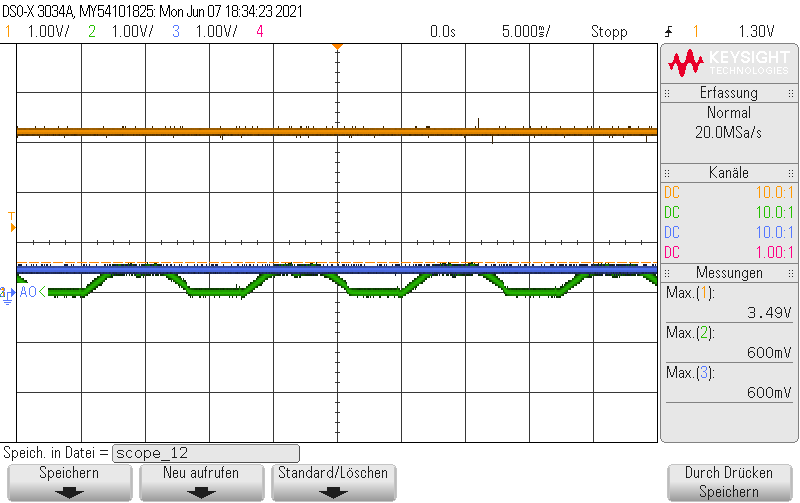
\includegraphics[width=.95\textwidth]{sec4/images/Problematik_stop_throttle} 
\centering
\captionsetup{width=.95\textwidth}
\caption[Fehlerhafte Rechtecksignal-Erzeugung bei niedrigen Drehzahlen]{Fehlerhafte Rechtecksignal-Erzeugung (in diesem Fall kein Rechteck) bei niedrigen Drehzahlen, wenn die Schaltschwellen nicht erreicht werden}\centering
\label{fig:ProblematikStopThrottle}
\end{figure}

Eine mögliche Lösung der Problematik ist die Erweiterung des Spannungsteilers für die Referenzspannung des OPV um eine zusätzliche und zuschaltbare Teilerstufe (1x für hohe Drehzahlen; 1x für niedrige Drehzahlen) mit einem n-Kanal MOSFET gegen Masse (siehe Abbildung \ref{fig:Schaltungserweiterung}). Diese Maßnahme ermöglicht es, die Referenzspannung, für hohe und niedrige Drehzahlen flexibel anzupassen um in jedem Fall ein zuverlässiges Ausgangssignal für die Messung der Drehzahl zu erhalten.\vspace{11pt}

Durch die Vorgabe eines bestimmten Modus (MCU-Mode), kann durch die Definition von zwei Drehzahlbereichen (z.B. Pulsbreite 1,09ms - 1,43ms langsam; Pulsbreite 1,43ms - 1,9ms schnell) eine individuelle Referenzspannung von ca. 500mV für langsame Drehzahlen und min. 1V für hohe Drehzahlen eingestellt werden. Der Vorteil ist, dass man dadurch einen bestimmten Toleranzbereich für Schwankungen der Versorgungsspannung erzeugt und die Schaltung dadurch weniger anfällig für Abweichungen ist.\vspace{11pt}

\begin{figure}[H] %H für Positionierung hier
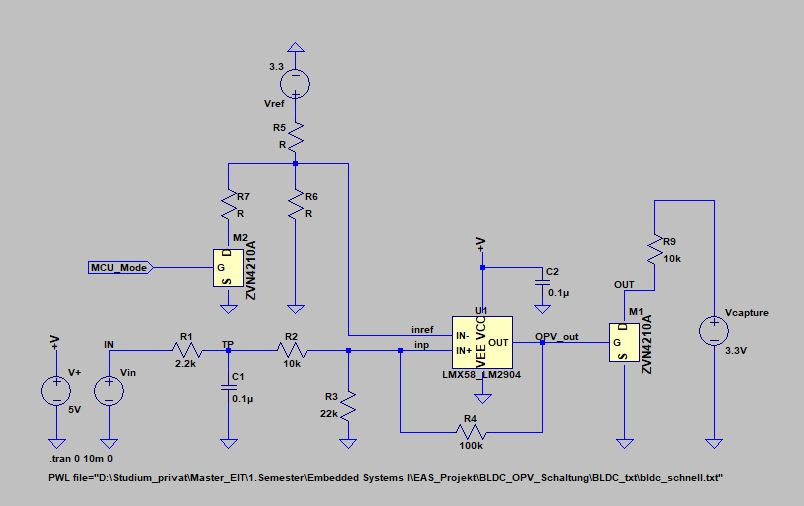
\includegraphics[width=.99\textwidth]{sec4/images/Schaltungserweiterung} 
\centering
\captionsetup{width=.95\textwidth}
\caption[Schaltplan der Tiefpass-/Komparatorschaltung nach der Schaltungserweiterung]{Schaltplan der Tiefpass-/Komparatorschaltung nach der Schaltungserweiterung um eine zweite Referenzspannungsstufe; erstellt für die Simulation eines Phasensignals in LTspice XVII}\centering
\label{fig:Schaltungserweiterung}
\end{figure}

In der Software muss hierzu in der Interrupt Service Routine der Drehzahlwert-Erfassung eine Umschalterkennung programmiert werden. Diese stellt über einen Ausgang des Mikrocontrollers die Referenzspannungsstufen über einen n-Kanal MOSFET so ein, wie sie bei der aktuellen Drehzahl gerade benötigt werden. Zur Bestimmung der Widerstandswerte für R5, R6 und R7 können die Gleichungen \ref{eq4.3} und \ref{eq4.4} verwendet werden.\vspace{11pt}

\begin{equation}\label{eq4.3}
V_{ModeLow} = \frac{ R6 }{R6 + R5 }\cdot 3,3V
\end{equation}

\begin{equation}\label{eq4.4}
V_{ModeHigh} = \frac{ R7 || R6 }{(R7 || R6) + R5}\cdot 3,3V
\end{equation}

\newpage
